\documentclass[]{book}
\usepackage{lmodern}
\usepackage{amssymb,amsmath}
\usepackage{ifxetex,ifluatex}
\usepackage{fixltx2e} % provides \textsubscript
\ifnum 0\ifxetex 1\fi\ifluatex 1\fi=0 % if pdftex
  \usepackage[T1]{fontenc}
  \usepackage[utf8]{inputenc}
\else % if luatex or xelatex
  \ifxetex
    \usepackage{mathspec}
  \else
    \usepackage{fontspec}
  \fi
  \defaultfontfeatures{Ligatures=TeX,Scale=MatchLowercase}
\fi
% use upquote if available, for straight quotes in verbatim environments
\IfFileExists{upquote.sty}{\usepackage{upquote}}{}
% use microtype if available
\IfFileExists{microtype.sty}{%
\usepackage{microtype}
\UseMicrotypeSet[protrusion]{basicmath} % disable protrusion for tt fonts
}{}
\usepackage[margin=1in]{geometry}
\usepackage{hyperref}
\PassOptionsToPackage{usenames,dvipsnames}{color} % color is loaded by hyperref
\hypersetup{unicode=true,
            pdftitle={Intro to Regression Analysis},
            pdfauthor={Maria Tackett},
            colorlinks=true,
            linkcolor=Maroon,
            citecolor=Blue,
            urlcolor=Blue,
            breaklinks=true}
\urlstyle{same}  % don't use monospace font for urls
\usepackage{natbib}
\bibliographystyle{apalike}
\usepackage{color}
\usepackage{fancyvrb}
\newcommand{\VerbBar}{|}
\newcommand{\VERB}{\Verb[commandchars=\\\{\}]}
\DefineVerbatimEnvironment{Highlighting}{Verbatim}{commandchars=\\\{\}}
% Add ',fontsize=\small' for more characters per line
\usepackage{framed}
\definecolor{shadecolor}{RGB}{248,248,248}
\newenvironment{Shaded}{\begin{snugshade}}{\end{snugshade}}
\newcommand{\KeywordTok}[1]{\textcolor[rgb]{0.13,0.29,0.53}{\textbf{#1}}}
\newcommand{\DataTypeTok}[1]{\textcolor[rgb]{0.13,0.29,0.53}{#1}}
\newcommand{\DecValTok}[1]{\textcolor[rgb]{0.00,0.00,0.81}{#1}}
\newcommand{\BaseNTok}[1]{\textcolor[rgb]{0.00,0.00,0.81}{#1}}
\newcommand{\FloatTok}[1]{\textcolor[rgb]{0.00,0.00,0.81}{#1}}
\newcommand{\ConstantTok}[1]{\textcolor[rgb]{0.00,0.00,0.00}{#1}}
\newcommand{\CharTok}[1]{\textcolor[rgb]{0.31,0.60,0.02}{#1}}
\newcommand{\SpecialCharTok}[1]{\textcolor[rgb]{0.00,0.00,0.00}{#1}}
\newcommand{\StringTok}[1]{\textcolor[rgb]{0.31,0.60,0.02}{#1}}
\newcommand{\VerbatimStringTok}[1]{\textcolor[rgb]{0.31,0.60,0.02}{#1}}
\newcommand{\SpecialStringTok}[1]{\textcolor[rgb]{0.31,0.60,0.02}{#1}}
\newcommand{\ImportTok}[1]{#1}
\newcommand{\CommentTok}[1]{\textcolor[rgb]{0.56,0.35,0.01}{\textit{#1}}}
\newcommand{\DocumentationTok}[1]{\textcolor[rgb]{0.56,0.35,0.01}{\textbf{\textit{#1}}}}
\newcommand{\AnnotationTok}[1]{\textcolor[rgb]{0.56,0.35,0.01}{\textbf{\textit{#1}}}}
\newcommand{\CommentVarTok}[1]{\textcolor[rgb]{0.56,0.35,0.01}{\textbf{\textit{#1}}}}
\newcommand{\OtherTok}[1]{\textcolor[rgb]{0.56,0.35,0.01}{#1}}
\newcommand{\FunctionTok}[1]{\textcolor[rgb]{0.00,0.00,0.00}{#1}}
\newcommand{\VariableTok}[1]{\textcolor[rgb]{0.00,0.00,0.00}{#1}}
\newcommand{\ControlFlowTok}[1]{\textcolor[rgb]{0.13,0.29,0.53}{\textbf{#1}}}
\newcommand{\OperatorTok}[1]{\textcolor[rgb]{0.81,0.36,0.00}{\textbf{#1}}}
\newcommand{\BuiltInTok}[1]{#1}
\newcommand{\ExtensionTok}[1]{#1}
\newcommand{\PreprocessorTok}[1]{\textcolor[rgb]{0.56,0.35,0.01}{\textit{#1}}}
\newcommand{\AttributeTok}[1]{\textcolor[rgb]{0.77,0.63,0.00}{#1}}
\newcommand{\RegionMarkerTok}[1]{#1}
\newcommand{\InformationTok}[1]{\textcolor[rgb]{0.56,0.35,0.01}{\textbf{\textit{#1}}}}
\newcommand{\WarningTok}[1]{\textcolor[rgb]{0.56,0.35,0.01}{\textbf{\textit{#1}}}}
\newcommand{\AlertTok}[1]{\textcolor[rgb]{0.94,0.16,0.16}{#1}}
\newcommand{\ErrorTok}[1]{\textcolor[rgb]{0.64,0.00,0.00}{\textbf{#1}}}
\newcommand{\NormalTok}[1]{#1}
\usepackage{longtable,booktabs}
\usepackage{graphicx,grffile}
\makeatletter
\def\maxwidth{\ifdim\Gin@nat@width>\linewidth\linewidth\else\Gin@nat@width\fi}
\def\maxheight{\ifdim\Gin@nat@height>\textheight\textheight\else\Gin@nat@height\fi}
\makeatother
% Scale images if necessary, so that they will not overflow the page
% margins by default, and it is still possible to overwrite the defaults
% using explicit options in \includegraphics[width, height, ...]{}
\setkeys{Gin}{width=\maxwidth,height=\maxheight,keepaspectratio}
\IfFileExists{parskip.sty}{%
\usepackage{parskip}
}{% else
\setlength{\parindent}{0pt}
\setlength{\parskip}{6pt plus 2pt minus 1pt}
}
\setlength{\emergencystretch}{3em}  % prevent overfull lines
\providecommand{\tightlist}{%
  \setlength{\itemsep}{0pt}\setlength{\parskip}{0pt}}
\setcounter{secnumdepth}{5}
% Redefines (sub)paragraphs to behave more like sections
\ifx\paragraph\undefined\else
\let\oldparagraph\paragraph
\renewcommand{\paragraph}[1]{\oldparagraph{#1}\mbox{}}
\fi
\ifx\subparagraph\undefined\else
\let\oldsubparagraph\subparagraph
\renewcommand{\subparagraph}[1]{\oldsubparagraph{#1}\mbox{}}
\fi

%%% Use protect on footnotes to avoid problems with footnotes in titles
\let\rmarkdownfootnote\footnote%
\def\footnote{\protect\rmarkdownfootnote}

%%% Change title format to be more compact
\usepackage{titling}

% Create subtitle command for use in maketitle
\providecommand{\subtitle}[1]{
  \posttitle{
    \begin{center}\large#1\end{center}
    }
}

\setlength{\droptitle}{-2em}

  \title{Intro to Regression Analysis}
    \pretitle{\vspace{\droptitle}\centering\huge}
  \posttitle{\par}
    \author{Maria Tackett}
    \preauthor{\centering\large\emph}
  \postauthor{\par}
      \predate{\centering\large\emph}
  \postdate{\par}
    \date{2019-05-13}

\usepackage{booktabs}

\begin{document}
\maketitle

{
\hypersetup{linkcolor=black}
\setcounter{tocdepth}{1}
\tableofcontents
}
\listoftables
\listoffigures
\chapter{Beginning of the Book}\label{beginning-of-the-book}

This is the introduction to the book.

This work is licensed under the
\href{http://creativecommons.org/licenses/by-nc-sa/4.0/}{Creative
Commons Attribution-NonCommercial-ShareAlike 4.0 International License}.

\chapter{Introduction}\label{intro}

You can label chapter and section titles using \texttt{\{\#label\}}
after them, e.g., we can reference Chapter \ref{intro}. If you do not
manually label them, there will be automatic labels anyway, e.g.,
Chapter \ref{methods}.

Figures and tables with captions will be placed in \texttt{figure} and
\texttt{table} environments, respectively.

\begin{Shaded}
\begin{Highlighting}[]
\KeywordTok{par}\NormalTok{(}\DataTypeTok{mar =} \KeywordTok{c}\NormalTok{(}\DecValTok{4}\NormalTok{, }\DecValTok{4}\NormalTok{, .}\DecValTok{1}\NormalTok{, .}\DecValTok{1}\NormalTok{))}
\KeywordTok{plot}\NormalTok{(pressure, }\DataTypeTok{type =} \StringTok{'b'}\NormalTok{, }\DataTypeTok{pch =} \DecValTok{19}\NormalTok{)}
\end{Highlighting}
\end{Shaded}

\begin{figure}

{\centering 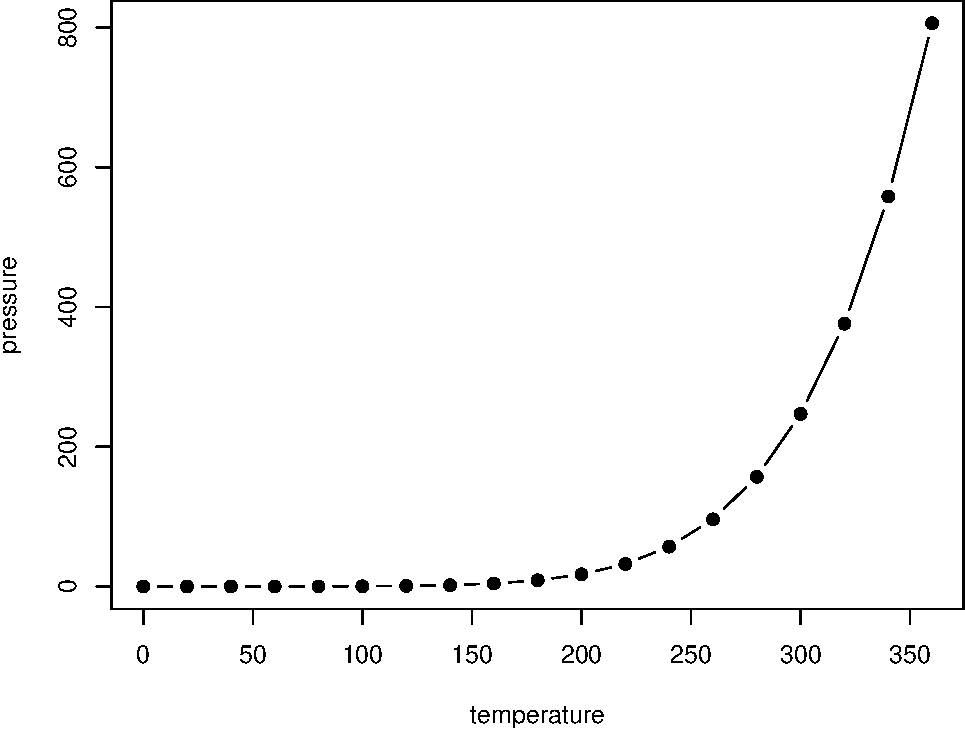
\includegraphics[width=0.8\linewidth]{introregression_files/figure-latex/nice-fig-1} 

}

\caption{Here is a nice figure!}\label{fig:nice-fig}
\end{figure}

Reference a figure by its code chunk label with the \texttt{fig:}
prefix, e.g., see Figure \ref{fig:nice-fig}. Similarly, you can
reference tables generated from \texttt{knitr::kable()}, e.g., see Table
\ref{tab:nice-tab}.

\begin{Shaded}
\begin{Highlighting}[]
\NormalTok{knitr}\OperatorTok{::}\KeywordTok{kable}\NormalTok{(}
  \KeywordTok{head}\NormalTok{(iris, }\DecValTok{20}\NormalTok{), }\DataTypeTok{caption =} \StringTok{'Here is a nice table!'}\NormalTok{,}
  \DataTypeTok{booktabs =} \OtherTok{TRUE}
\NormalTok{)}
\end{Highlighting}
\end{Shaded}

\begin{table}[t]

\caption{\label{tab:nice-tab}Here is a nice table!}
\centering
\begin{tabular}{rrrrl}
\toprule
Sepal.Length & Sepal.Width & Petal.Length & Petal.Width & Species\\
\midrule
5.1 & 3.5 & 1.4 & 0.2 & setosa\\
4.9 & 3.0 & 1.4 & 0.2 & setosa\\
4.7 & 3.2 & 1.3 & 0.2 & setosa\\
4.6 & 3.1 & 1.5 & 0.2 & setosa\\
5.0 & 3.6 & 1.4 & 0.2 & setosa\\
\addlinespace
5.4 & 3.9 & 1.7 & 0.4 & setosa\\
4.6 & 3.4 & 1.4 & 0.3 & setosa\\
5.0 & 3.4 & 1.5 & 0.2 & setosa\\
4.4 & 2.9 & 1.4 & 0.2 & setosa\\
4.9 & 3.1 & 1.5 & 0.1 & setosa\\
\addlinespace
5.4 & 3.7 & 1.5 & 0.2 & setosa\\
4.8 & 3.4 & 1.6 & 0.2 & setosa\\
4.8 & 3.0 & 1.4 & 0.1 & setosa\\
4.3 & 3.0 & 1.1 & 0.1 & setosa\\
5.8 & 4.0 & 1.2 & 0.2 & setosa\\
\addlinespace
5.7 & 4.4 & 1.5 & 0.4 & setosa\\
5.4 & 3.9 & 1.3 & 0.4 & setosa\\
5.1 & 3.5 & 1.4 & 0.3 & setosa\\
5.7 & 3.8 & 1.7 & 0.3 & setosa\\
5.1 & 3.8 & 1.5 & 0.3 & setosa\\
\bottomrule
\end{tabular}
\end{table}

You can write citations, too. For example, we are using the
\textbf{bookdown} package \citep{R-bookdown} in this sample book, which
was built on top of R Markdown and \textbf{knitr} \citep{xie2015}.

\chapter{Getting Started}\label{getstarted}

I am updating this to test it out.

\part{Assignments}\label{part-assignments}

\chapter{Intro to R}\label{intro-to-r}

\section{Introduction}\label{introduction}

\begin{Shaded}
\begin{Highlighting}[]
\CommentTok{# R is the name of the programming language itself and RStudio is a convenient interface.}
\end{Highlighting}
\end{Shaded}

The main goal of this lab is to introduce you to R and RStudio, which we
will be using throughout the course both to learn the statistical
concepts discussed in the course and to analyze real data and come to
informed conclusions.

\begin{Shaded}
\begin{Highlighting}[]
\CommentTok{# git is a version control system (like "Track Changes" features from Microsoft Word but more powerful) and GitHub is the home for your Git-based projects on the internet (like DropBox but much better).}
\end{Highlighting}
\end{Shaded}

An additional goal is to introduce you to git and GitHub, which is the
collaboration and version control system that we will be using
throughout the course.

As the labs progress, you are encouraged to explore beyond what the labs
dictate; a willingness to experiment will make you a much better
programmer and statistician. If you're new to R, you should begin by
building some basic fluency in R. Today's lab will focus on fundamental
building blocks of R and RStudio: the interface, reading in data, and
basic commands. Starting next week, the labs will focus on concepts more
specific to regression analysis.

To make versioning simpler, today's lab is individual. This will give
you a chance to become more familiar with git and GitHub. Next week
you'll learn about collaborating on GitHub and will produce a single lab
report as a team.

\subsection{Topics covered in this
lab:}\label{topics-covered-in-this-lab}

\begin{itemize}
\tightlist
\item
  Exploratory Data Analysis (data visualizations and numerical
  summaries)
\item
  Simple linear regression
\item
  Writing a lab report using R Markdown
\item
  Tracking changes and submitting work using git and GitHub
\end{itemize}

\section{Packages}\label{packages}

We will use the following packages in today's lab.

\begin{Shaded}
\begin{Highlighting}[]
\KeywordTok{library}\NormalTok{(tidyverse)}
\KeywordTok{library}\NormalTok{(readr)}
\KeywordTok{library}\NormalTok{(skimr)}
\KeywordTok{library}\NormalTok{(broom)}
\end{Highlighting}
\end{Shaded}

If you need to install any of the packages, you can run the code below
in the \textbf{console}.

\begin{Shaded}
\begin{Highlighting}[]
\KeywordTok{install.packages}\NormalTok{(}\StringTok{"tidyverse"}\NormalTok{) }
\KeywordTok{install.packages}\NormalTok{(}\StringTok{"readr"}\NormalTok{)}
\KeywordTok{install.packages}\NormalTok{(}\StringTok{"skimr"}\NormalTok{)}
\KeywordTok{install.packages}\NormalTok{(}\StringTok{"broom"}\NormalTok{)}
\end{Highlighting}
\end{Shaded}

\section{Warm up}\label{warm-up}

Before we introduce the data, let's warm up with some simple exercises.

\section{Project name:}\label{project-name}

Currently your project is called \emph{Untitled Project}. Update the
name of your project to be ``Lab 01 - Intro R''.

\begin{Shaded}
\begin{Highlighting}[]
\CommentTok{# The top portion of your R Markdown file (between the three dashed lines) is called YAML. It stands for "YAML Ain't Markup Language". It is a human friendly data serialization standard for all programming languages. All you need to know is that this area is called the YAML (we will refer to it as such) and that it contains meta information about your document.}
\end{Highlighting}
\end{Shaded}

\subsection{YAML:}\label{yaml}

Open the R Markdown (Rmd) file in your project, change the author name
to your name, and knit the document.

\subsection{Commiting changes:}\label{commiting-changes}

Then go to the Git pane in your RStudio.

If you have made changes to your Rmd file, you should see it listed
here. Click on it to select it in this list and then click on
\textbf{Diff}. This shows you the \emph{diff}erence between the last
committed state of the document and its current state that includes your
changes. If you're happy with these changes, write ``Update author
name'' in the \textbf{Commit message} box and click \textbf{Commit}.

You don't have to commit after every change, this would get quite
cumbersome. You should consider committing states that are
\emph{meaningful to you} for inspection, comparison, or restoration. In
the first few assignments we will tell you exactly when to commit and in
some cases, what commit message to use. As the semester progresses we
will let you make these decisions.

\subsection{Pushing changes:}\label{pushing-changes}

Now that you have made an update and committed this change, it's time to
push these changes to the web! Or more specifically, to your repo on
GitHub. Why? So that others can see your changes. And by others, we mean
the course teaching team (your repos in this course are private to you
and us, only).

In order to push your changes to GitHub, click on \textbf{Push}. This
will prompt a dialogue box where you first need to enter your user name,
and then your password. This might feel cumbersome. Bear with me\ldots{}
We \emph{will} teach you how to save your password so you don't have to
enter it every time. But for this one assignment you'll have to manually
enter each time you push in order to gain some experience with it.

\subsection{Data}\label{data}

Today's data comes from the Capital Bikeshare in Washington D.C. The
Capital Bikeshare is a system in which customers can rent a bike for
little cost, ride it around the city, and return it to a station near
their destination. You can get more information about the bikeshare on
their website, \url{https://www.capitalbikeshare.com/}. We will read in
the data from the file \emph{bikeshare.csv} located in the \emph{data}
folder.

\begin{Shaded}
\begin{Highlighting}[]
\NormalTok{bikeshare <-}\StringTok{ }\KeywordTok{read_csv}\NormalTok{(}\StringTok{"data/bikeshare.csv"}\NormalTok{)}
\end{Highlighting}
\end{Shaded}

This dataset contains information about the number of bike rentals,
environmental conditions, and other information about the each day in
2011 and 2012.

\section{Exercises}\label{exercises}

Before doing any analysis, we want to understand the basic structure of
the data. One way to do this, is to look at the actual dataset. Type the
code below in the \textbf{console} to view the entire dataset.

\begin{Shaded}
\begin{Highlighting}[]
\KeywordTok{View}\NormalTok{(bikeshare)}
\end{Highlighting}
\end{Shaded}

It is sometimes more useful to view a summary of the data structure
rather than view the entire dataset. This is especially true for very
large datasets, i.e.~those with a very large number of observations
and/or rows. We can use the \texttt{glimpse()} function to get a general
idea about the structure of our dataset. This function can be very
useful when importing data from a file such as a .csv file (like in this
lab) to ensure that data imported correctly and that we have the number
of observations (rows) and variables (columns) we expect. We can also
use this function to see each variable's type (e.g.~integer, character).

\begin{Shaded}
\begin{Highlighting}[]
\CommentTok{# You can  type `??glimpse` in the console to learn more about the function and its syntax.}
\end{Highlighting}
\end{Shaded}

\begin{enumerate}
\def\labelenumi{\arabic{enumi}.}
\tightlist
\item
  Type \texttt{glimpse(bikeshare)} in the \textbf{console} an overview
  of the \texttt{bikeshare} dataset.
\end{enumerate}

How many observations are in the \texttt{bikeshare} dataset? How many
variables?

\begin{enumerate}
\def\labelenumi{\arabic{enumi}.}
\setcounter{enumi}{1}
\tightlist
\item
  In this lab, we will focus the analysis on the following variables:
\end{enumerate}

\begin{longtable}[]{@{}ll@{}}
\toprule
\texttt{season} & 1: Winter, 2: Spring, 3: Summer, 4:
Fall\tabularnewline
\texttt{temp} & Temperature (in \(^{\circ}C\)) ÷ 41\tabularnewline
\texttt{count} & total number of bike rentals\tabularnewline
\bottomrule
\end{longtable}

Before fitting any regression models, we want to do an exploratory data
analysis (EDA) to summarize the main characteristics of the data. Much
of the EDA is visual, which we'll get to in the next exercise. The EDA
also consists of calculating summary statistics for the variables in our
dataset. It is good practice to examine any variable that may be
relevant to the analysis in the EDA, since there may be variables that
aren't directly included in the regression model but are still affecting
the results. To keep today's lab manageable, we will only examine the
three variables \texttt{season}, \texttt{temp}, and \texttt{count}.

There are many ways to calculate summary statistics for each variable,
and we will use a few of them throughout the semester. For now, let's
use the \texttt{skim()} function to calculate basic measures of center
and spread along with get a sketch of the distribution.

\begin{Shaded}
\begin{Highlighting}[]
\NormalTok{bikeshare }\OperatorTok
\StringTok{  }\KeywordTok{select}\NormalTok{(season,temp,count) }\OperatorTok
\StringTok{  }\KeywordTok{skim}\NormalTok{()}
\end{Highlighting}
\end{Shaded}

What is the mean number of bike rentals? About 25\% of the days in the
data have a \texttt{count} above what value?

\begin{enumerate}
\def\labelenumi{\arabic{enumi}.}
\setcounter{enumi}{2}
\tightlist
\item
  Does it make sense to calculate measures of center and spread for the
  variable \texttt{season}? If so, explain why it makes sense.
  Otherwise, explain why the \texttt{skim()} function calculated these
  summary statistics for the variable \texttt{season} even if they don't
  make sense.
\end{enumerate}

\emph{This is a good place to pause and commit changes with the commit
message ``Added summary statistics (Ex 1 - 3)'', and push.}

\subsection{Visualizing Your Data}\label{visualizing-your-data}

\begin{enumerate}
\def\labelenumi{\arabic{enumi}.}
\setcounter{enumi}{3}
\tightlist
\item
  One important part of EDA is visualizing the data to get a better idea
  of the shape of the distribution of each variable along with the
  relationship between variables. There are a lot of ways to make plots
  in R; we will use the functions available in the \texttt{ggplot2}
  package.
\end{enumerate}

The code below is used to create a histogram to visualize the
distribution of \texttt{count}. Modify the code by writing an
informative title and label for the x-axis.

\begin{Shaded}
\begin{Highlighting}[]
\KeywordTok{ggplot}\NormalTok{(}\DataTypeTok{data=}\NormalTok{bikeshare, }\DataTypeTok{mapping=}\KeywordTok{aes}\NormalTok{(}\DataTypeTok{x=}\NormalTok{count)) }\OperatorTok{+}\StringTok{ }
\StringTok{  }\KeywordTok{geom_histogram}\NormalTok{() }\OperatorTok{+}
\StringTok{  }\KeywordTok{labs}\NormalTok{(}\DataTypeTok{title=}\StringTok{"______"}\NormalTok{, }\DataTypeTok{x=}\StringTok{"______"}\NormalTok{)}
\end{Highlighting}
\end{Shaded}

\begin{enumerate}
\def\labelenumi{\arabic{enumi}.}
\setcounter{enumi}{4}
\tightlist
\item
  Sometimes you may want to customize a plot by changing different
  features such as the color, marker types, etc. When plotting a
  histogram, one easy way to customize it is by changing the color the
  bars. We'll look at two different ways to do this.
\end{enumerate}

First, using a color of your choice, include the option
\texttt{color="\_\_\_\_\_"} inside of \texttt{geom\_histogram()}
function. Your code will look similar this. Be sure to also include an
informative title and label for the x-axis.

\begin{Shaded}
\begin{Highlighting}[]
\KeywordTok{ggplot}\NormalTok{(}\DataTypeTok{data=}\NormalTok{bikeshare, }\DataTypeTok{mapping=}\KeywordTok{aes}\NormalTok{(}\DataTypeTok{x=}\NormalTok{count)) }\OperatorTok{+}\StringTok{ }
\StringTok{  }\KeywordTok{geom_histogram}\NormalTok{(}\DataTypeTok{color=}\StringTok{"_______"}\NormalTok{) }\OperatorTok{+}
\StringTok{  }\KeywordTok{labs}\NormalTok{(}\DataTypeTok{title=}\StringTok{"______"}\NormalTok{, }\DataTypeTok{x=}\StringTok{"______"}\NormalTok{)}
\end{Highlighting}
\end{Shaded}

\begin{Shaded}
\begin{Highlighting}[]
\CommentTok{# This [ggplot2 quick reference](http://sape.inf.usi.ch/quick-reference/ggplot2/colour) has a long list of color options. You can also use [HTML color codes](https://htmlcolorcodes.com/).}
\end{Highlighting}
\end{Shaded}

Next, instead of \texttt{color="\_\_\_\_\_"}, use
\texttt{fill="\_\_\_\_\_\_"} inside of the \texttt{geom\_histogram()}
function and put the color of your choice inside the blank. You can use
the same color as before or use a new one.

What is the difference in the two plots? In other words, what is the
difference in the way color is implemented when using \texttt{color}
versus \texttt{fill}?

\begin{enumerate}
\def\labelenumi{\arabic{enumi}.}
\setcounter{enumi}{5}
\tightlist
\item
  Describe the distribution of \texttt{count}. Your description should
  include comments about the shape, center, spread, and any potential
  outliers. You should use the histogram and the summary statistics from
  Exercise 2 in your description.
\end{enumerate}

\emph{This is a another good place to pause and commit changes with the
commit message ``Added data visualization of count (Ex 3 - 6)'', and
push.}

\begin{enumerate}
\def\labelenumi{\arabic{enumi}.}
\setcounter{enumi}{6}
\tightlist
\item
  Now that we've examined the variables individually, we want to look at
  the relationship between the variables. To make interpretation easier,
  we will use the \texttt{mutate()} function to create a new variable
  called \texttt{temp\_c} that is calculated as \texttt{temp\ *\ 41}. We
  will use \texttt{temp\_c} for the remainder of the analysis, so the
  temperature can be discussed in terms of degrees Celsius.
\end{enumerate}

\begin{Shaded}
\begin{Highlighting}[]
\NormalTok{bikeshare <-}\StringTok{ }\NormalTok{bikeshare }\OperatorTok
\StringTok{  }\KeywordTok{mutate}\NormalTok{(}\DataTypeTok{temp_c =}\NormalTok{ temp }\OperatorTok{*}\StringTok{ }\DecValTok{41}\NormalTok{)}
\end{Highlighting}
\end{Shaded}

Complete the code below to make a scatterplot of the number of bike
rentals versus the temperature.

\begin{Shaded}
\begin{Highlighting}[]
\KeywordTok{ggplot}\NormalTok{(}\DataTypeTok{data=}\NormalTok{bikeshare, }\DataTypeTok{mapping=}\KeywordTok{aes}\NormalTok{(}\DataTypeTok{x=}\NormalTok{temp_c,}\DataTypeTok{y=}\NormalTok{count)) }\OperatorTok{+}
\StringTok{  }\NormalTok{___________________}
\end{Highlighting}
\end{Shaded}

\begin{Shaded}
\begin{Highlighting}[]
\CommentTok{# [https://ggplot2.tidyverse.org/](https://ggplot2.tidyverse.org/) is a great resource as you learn `ggplot()`. Click **Reference** in the top right corner to see a list of the various plot types available in the ggplot2 package.}
\end{Highlighting}
\end{Shaded}

Describe the relationship between the temperature and the number of bike
rentals.

\begin{enumerate}
\def\labelenumi{\arabic{enumi}.}
\setcounter{enumi}{7}
\tightlist
\item
  The temperature and number of bike rentals varies greatly depending on
  the season. Therefore, we would like to create a separate scatterplot
  of \texttt{count} versus \texttt{temp\_c} for each season. To do so,
  we will use the \texttt{facet\_wrap()} function, faceting by
  \texttt{season}. Recall from Exercise 2 that \texttt{season} is
  currently stored as an integer. We need to change it to a factor
  variable type before using it in the \texttt{facet\_wrap()} function
  (you could also change it to a character variable).
\end{enumerate}

\begin{Shaded}
\begin{Highlighting}[]
\NormalTok{bikeshare <-}\StringTok{ }\NormalTok{bikeshare }\OperatorTok
\StringTok{  }\KeywordTok{mutate}\NormalTok{(}\DataTypeTok{season =} \KeywordTok{as.factor}\NormalTok{(season))}
\end{Highlighting}
\end{Shaded}

\begin{Shaded}
\begin{Highlighting}[]
\KeywordTok{ggplot}\NormalTok{(}\DataTypeTok{data=}\NormalTok{bikeshare, }\DataTypeTok{mapping=}\KeywordTok{aes}\NormalTok{(}\DataTypeTok{x=}\NormalTok{temp_c,}\DataTypeTok{y=}\NormalTok{count)) }\OperatorTok{+}\StringTok{ }
\StringTok{  }\KeywordTok{geom_point}\NormalTok{() }\OperatorTok{+}
\StringTok{  }\KeywordTok{labs}\NormalTok{(}\DataTypeTok{title =} \StringTok{"Number of Bike Rentals vs. Temperature"}\NormalTok{, }
       \DataTypeTok{subtitle=}\StringTok{"Faceted by Season"}\NormalTok{, }
       \DataTypeTok{x =} \StringTok{"Temperature (Celsius)"}\NormalTok{, }
       \DataTypeTok{y =} \StringTok{"Number of Bike Rentals"}\NormalTok{) }\OperatorTok{+}
\StringTok{  }\KeywordTok{facet_wrap}\NormalTok{(}\OperatorTok{~}\NormalTok{season)}
\end{Highlighting}
\end{Shaded}

For which season does the linear relationship between the temperature
and the number of bike rentals appear to be the strongest?

\emph{This is a another good place to pause and commit changes with the
commit message ``Added visualization of count vs.~temperature (Ex 7 -
8)'', and push.}

\section{Simple Linear Regression}\label{simple-linear-regression}

We want to fit a least-squares regression using the temperature
(\texttt{temp\_c}) to explain variation in the number of bike rentals
(\texttt{count}) in the \textbf{winter} season. We can use the
\texttt{filter()} function to create a subset from the data that only
includes days during the winter. The \texttt{\textless{}-} assigns the
name \texttt{winter\_data} to our subset.

\begin{Shaded}
\begin{Highlighting}[]
\NormalTok{winter_data <-}\StringTok{ }\NormalTok{bikeshare }\OperatorTok
\StringTok{  }\KeywordTok{filter}\NormalTok{(season}\OperatorTok{==}\StringTok{"1"}\NormalTok{)}
\end{Highlighting}
\end{Shaded}

We will use \texttt{winter\_data} for the remainder of the lab.

\begin{enumerate}
\def\labelenumi{\arabic{enumi}.}
\setcounter{enumi}{8}
\tightlist
\item
  Fit a simple linear regression model with using the \texttt{lm()}
  function; assign it the name \texttt{winter\_model}. Replace \emph{X},
  \emph{Y}, and \emph{my.data} in the code below with the appropriate
  values.
\end{enumerate}

\begin{Shaded}
\begin{Highlighting}[]
\NormalTok{winter_model <-}\StringTok{ }\KeywordTok{lm}\NormalTok{(Y }\OperatorTok{~}\StringTok{ }\NormalTok{X, }\DataTypeTok{data=}\NormalTok{my.data)}
\KeywordTok{tidy}\NormalTok{(model) }\CommentTok{#output model}
\end{Highlighting}
\end{Shaded}

Interpret the slope.

Does it make sense to interpret the intercept? If so, write the
interpretation of the intercept. Otherwise, explain why not.

\begin{enumerate}
\def\labelenumi{\arabic{enumi}.}
\setcounter{enumi}{9}
\tightlist
\item
  We conclude by checking the assumptions for regression. We use the
  \texttt{mutate()} function to add a new variable called \texttt{resid}
  that is the residual for each observation in \texttt{winter\_data}
  data.
\end{enumerate}

\begin{Shaded}
\begin{Highlighting}[]
\NormalTok{winter_data <-}\StringTok{ }\NormalTok{winter_data }\OperatorTok
\StringTok{  }\KeywordTok{mutate}\NormalTok{(}\DataTypeTok{resid =} \KeywordTok{residuals}\NormalTok{(winter_model))}
\end{Highlighting}
\end{Shaded}

The code for the residuals vs.~the predictor variable and the Normal QQ
plot are below. In addition to these plots, write the code to make a
histogram of the residuals. You can reuse code from a previous exercise
to plot the histogram.

\begin{Shaded}
\begin{Highlighting}[]
\KeywordTok{ggplot}\NormalTok{(}\DataTypeTok{data=}\NormalTok{winter_data, }\DataTypeTok{mapping=}\KeywordTok{aes}\NormalTok{(}\DataTypeTok{x=}\NormalTok{temp_c,}\DataTypeTok{y=}\NormalTok{resid)) }\OperatorTok{+}
\StringTok{  }\KeywordTok{geom_point}\NormalTok{() }\OperatorTok{+}\StringTok{ }
\StringTok{  }\KeywordTok{geom_hline}\NormalTok{(}\DataTypeTok{yintercept=}\DecValTok{0}\NormalTok{,}\DataTypeTok{color=}\StringTok{"red"}\NormalTok{)}\OperatorTok{+}
\StringTok{  }\KeywordTok{labs}\NormalTok{(}\DataTypeTok{title=}\StringTok{"Residuals vs. Temperature"}\NormalTok{,}
       \DataTypeTok{x=}\StringTok{"Temperature"}\NormalTok{, }
       \DataTypeTok{y=}\StringTok{"Residuals"}\NormalTok{)}
\end{Highlighting}
\end{Shaded}

\begin{Shaded}
\begin{Highlighting}[]
\KeywordTok{ggplot}\NormalTok{(}\DataTypeTok{data=}\NormalTok{winter_data, }\DataTypeTok{mapping=}\KeywordTok{aes}\NormalTok{(}\DataTypeTok{sample=}\NormalTok{resid)) }\OperatorTok{+}
\StringTok{  }\KeywordTok{stat_qq}\NormalTok{() }\OperatorTok{+}\StringTok{ }
\StringTok{  }\KeywordTok{stat_qq_line}\NormalTok{()}\OperatorTok{+}
\StringTok{  }\KeywordTok{labs}\NormalTok{(}\DataTypeTok{title=}\StringTok{"Normal QQ Plot of Residuals"}\NormalTok{)}
\end{Highlighting}
\end{Shaded}

Based on the plots of the residuals and the scatterplot, are linearity,
normality, and constant variance assumptions met? Briefly explain.

Is the independence assumption met based on the description of the data?
Briefly explain.

\textbf{Optional:} Create a plot that could be used to help you assess
the independence assumption.

Throughout the semester, we will learn various methods to deal with any
violations in regression assumptions. For now, we will just note them.

\emph{You're done! Commit all remaining changes, use the commit message
``Done with Lab 1!'', and push. Before you wrap up the assignment, make
sure all documents are updated on your GitHub repo.}

\chapter{Simple Linear Regression}\label{slr}

The primary goal of today's lab is to give you practice with some of the
tools you will need to conduct regression analysis using R. An
additional goal for today is for you to be introduced to your teams and
practice collaborating using GitHub and RStudio.

\subsection{Packages}\label{packages-1}

We will use the following packages in today's lab.

\begin{Shaded}
\begin{Highlighting}[]
\KeywordTok{library}\NormalTok{(tidyverse)}
\KeywordTok{library}\NormalTok{(skimr)}
\KeywordTok{library}\NormalTok{(broom)}
\KeywordTok{library}\NormalTok{(rcfss)}
\end{Highlighting}
\end{Shaded}

\subsection{Project name:}\label{project-name-1}

Currently your project is called \emph{Untitled Project}. Update the
name of your project to be ``Lab 02 - Simple Linear Regression''

\section{Warm up}\label{warm-up-1}

\textbf{Pick one team member to complete the steps in this section while
the others contribute to the discussion but do not actually touch the
files on their computer.}

Before we introduce the data, let's warm up with a simple exercise.

\subsection{YAML:}\label{yaml-1}

Open the R Markdown (Rmd) file in your project, change the author name
to your \textbf{team} name, and knit the document.

\subsection{Commiting and pushing
changes:}\label{commiting-and-pushing-changes}

\begin{itemize}
\tightlist
\item
  Go to the \textbf{Git} pane in your RStudio.
\item
  View the \textbf{Diff} and confirm that you are happy with the
  changes.
\item
  Add a commit message like ``Update team name'' in the \textbf{Commit
  message} box and hit \textbf{Commit}.
\item
  Click on \textbf{Push}. This will prompt a dialogue box where you
  first need to enter your user name, and then your password.
\end{itemize}

\subsection{Pulling changes:}\label{pulling-changes}

Now, the remaining team members who have not been concurrently making
these changes on their projects should click on the \textbf{Pull} button
in their Git pane and observe that the changes are now reflected on
their projects as well.

\subsection{Data}\label{data-1}

In today's lab, we will analyze the \texttt{scorecard} dataset from the
rcfss package. This dataset contains information about 1849 colleges
obtained from the Department of Education's College Scorecard. Load the
rcfss library into the global R environment and type \texttt{?scorecard}
in the \textbf{console} to learn more about the dataset and variable
definitions. Today's analysis will focus on the following variables:

\begin{longtable}[]{@{}ll@{}}
\toprule
\begin{minipage}[t]{0.16\columnwidth}\raggedright\strut
\texttt{type}\strut
\end{minipage} & \begin{minipage}[t]{0.56\columnwidth}\raggedright\strut
Type of college (Public, Private - nonprofit, Private - for
profit)\strut
\end{minipage}\tabularnewline
\begin{minipage}[t]{0.16\columnwidth}\raggedright\strut
\texttt{cost}\strut
\end{minipage} & \begin{minipage}[t]{0.56\columnwidth}\raggedright\strut
The average annual cost of attendance, including tuition and feeds,
books and supplies, and living expenses, minus the average
grant/scholarship aid\strut
\end{minipage}\tabularnewline
\begin{minipage}[t]{0.16\columnwidth}\raggedright\strut
\texttt{admrate}\strut
\end{minipage} & \begin{minipage}[t]{0.56\columnwidth}\raggedright\strut
Undergraduate admissions rate (from 0 - 100\%)\strut
\end{minipage}\tabularnewline
\bottomrule
\end{longtable}

\section{Exercises}\label{exercises-1}

\subsection{Exploratory Data Analysis}\label{exploratory-data-analysis}

\begin{enumerate}
\def\labelenumi{\arabic{enumi}.}
\item
  Plot a histogram to examine the distribution of \texttt{admrate}. What
  is the shape of the distribution?
\item
  To better understand the distribution of \texttt{admrate}, we would
  like calculate measures of center and spread of the distribution. Fill
  in the code below to use the \texttt{skim} function to calculate
  summary statistics for \texttt{admrate}. Report the appropriate
  measures of center (mean or median) and spread (standard deviation or
  IQR) based on the shape of the distribution from Exercise 1.
\end{enumerate}

\begin{Shaded}
\begin{Highlighting}[]
\NormalTok{scorecard }\OperatorTok
\StringTok{  }\KeywordTok{select}\NormalTok{(admrate) }\OperatorTok
\StringTok{  }\KeywordTok{skim}\NormalTok{()}
\end{Highlighting}
\end{Shaded}

\begin{enumerate}
\def\labelenumi{\arabic{enumi}.}
\setcounter{enumi}{2}
\item
  Plot the distribution of \texttt{cost} and calculate the appropriate
  summary statistics. Describe the distribution of \texttt{cost} (shape,
  center, and spread) using the plot and appropriate summary statistics.
\item
  One nice feature of the \texttt{skim} function is that it provides
  information about the number of observations that are missing values
  of the variable. How many observations have missing values of
  \texttt{admrate}? How many observations have missing values of
  \texttt{cost}?
\item
  Later in the semester, we will techniques to deal with missing values
  in the data. For now, however, we will only include complete
  observations for the remainder of this analysis. We can use the
  \texttt{filter} function to select only the rows that values for both
  \texttt{cost} and \texttt{admrate}.
\end{enumerate}

Fill in the code below to create a new dataset called
\texttt{scorecard\_new} that only includes observations with values for
both \texttt{admrate} and \texttt{cost}.

\begin{Shaded}
\begin{Highlighting}[]
\NormalTok{__________ <-}\StringTok{ }\NormalTok{scorecard }\OperatorTok
\StringTok{  }\KeywordTok{filter}\NormalTok{(}\OperatorTok{!}\KeywordTok{is.na}\NormalTok{(admrate),________)}
\end{Highlighting}
\end{Shaded}

\begin{Shaded}
\begin{Highlighting}[]
\CommentTok{# Learn more about the `filter` function in [Section 5.2 of R for Data Science] (https://r4ds.had.co.nz/transform.html#filter-rows-with-filter)}
\end{Highlighting}
\end{Shaded}

You will use \texttt{scorecard\_new} for the rest of the lab.

\begin{enumerate}
\def\labelenumi{\arabic{enumi}.}
\setcounter{enumi}{5}
\item
  Create a scatterplot to display the relationship between \texttt{cost}
  (response variable) and \texttt{admrate} (explanatory variable). Use
  the scatterplot to describe the relationship between the two
  variables.
\item
  The data contains information about the type of college, and we would
  like to incorporate this information into the scatterplot. One way to
  do this is to use a different color marker for each type of college.
  Fill in the code below the scatterplot from the previous exercise with
  the marker colors based on the variable \texttt{type}. Describe two
  new observations from this scatterplot that you didn't see in the
  previous plot.
\end{enumerate}

\begin{Shaded}
\begin{Highlighting}[]
\KeywordTok{ggplot}\NormalTok{(}\DataTypeTok{data=}\NormalTok{scorecard_new, }\DataTypeTok{mapping=}\KeywordTok{aes}\NormalTok{(}\DataTypeTok{x=}\NormalTok{admrate, }\DataTypeTok{y=}\NormalTok{cost, }\DataTypeTok{color=}\NormalTok{type)) }\OperatorTok{+}\StringTok{ }
\StringTok{  }\NormalTok{_____________________}
\end{Highlighting}
\end{Shaded}

\subsection{Simple Linear Regression}\label{simple-linear-regression-1}

\begin{enumerate}
\def\labelenumi{\arabic{enumi}.}
\setcounter{enumi}{7}
\item
  Fit a regression model to describe the relationship between a
  college's admission rate and cost. Use the \texttt{tidy} function to
  display the model.
\item
  Interpret the slope in the context of the problem. Does the intercept
  have a meaningful interpretation? If so, write the interpretation in
  the context of the problem. Otherwise, explain why the interpretation
  is not meaningful.
\item
  While the \texttt{tidy} function is used to display the model, we can
  obtain a one-row summary of the model using the \texttt{glance}
  function. Use the \texttt{glance} function to get a summary of the
  model fit in the previous exercise. See the
  \href{https://rdrr.io/cran/broom/man/glance.lm.html}{documentation for
  \texttt{glance}} for the syntax and a list of values output from the
  function.
\item
  What is the value of \(R^2\)? Interpret this value in the context of
  the problem. Do you think this is a ``good'' value of \(R^2\)?
  Explain.
\item
  What is the value of \(\hat{\sigma}\), the residual standard error.
\item
  What is the 95\% confidence interval for the coefficient of
  \texttt{admrate}, i.e.~the slope? Interpret the interval in the
  context of the data.
\item
  We want to test the following hypotheses about the population slope
  \(\beta_1\):
\end{enumerate}

\[H_0: \beta_1 = 0 \hspace{5mm} \text{versus} \hspace{5mm} H_a: \beta_1 \neq 0\]

State what the null and alternative hypotheses mean in terms of the
linear relationship between \texttt{admrate} and \texttt{cost}.

\begin{enumerate}
\def\labelenumi{\arabic{enumi}.}
\setcounter{enumi}{14}
\tightlist
\item
  Consider the confidence interval from Exercise 13 and the hypotheses
  in Exercise 14. Is the confidence interval consistent with the null or
  alternative hypothesis? Briefly explain.
\end{enumerate}

\emph{You're done! Commit all remaining changes, use the commit message
``Done with Lab 2!'', and push. Before you wrap up the assignment, make
sure the .Rmd, .html, and .md documents are all updated on your GitHub
repo.}

\chapter{ANOVA}\label{anova}

The goal of this lab is to use Analysis of Variance (ANOVA) to compare
means in multiple groups. Additionally, you will be introduced to new R
functions used for
\href{https://en.wikipedia.org/wiki/Data_wrangling}{wrangling} and
summarizing data.

\subsection{Packages}\label{packages-2}

We will use the following packages in today's lab.

\begin{Shaded}
\begin{Highlighting}[]
\KeywordTok{library}\NormalTok{(tidyverse)}
\KeywordTok{library}\NormalTok{(knitr)}
\KeywordTok{library}\NormalTok{(broom)}
\end{Highlighting}
\end{Shaded}

\subsection{Data}\label{data-2}

In today's lab, we will analyze the \texttt{diamonds} dataset from the
ggplot2 package. Type \texttt{?diamonds} in the console to see a
dictionary of the variables in the data set. This analysis will focus on
the relationship between a diamond's carat weight and its color. Before
starting the exercises, take a moment to read more about the diamond
attributes on the Gemological Institute of America webpage:
\url{https://www.gia.edu/diamond-quality-factor}.

\section{Exercises}\label{exercises-2}

The diamonds dataset contains the price and other characteristics for
over 50,000 diamonds price from \$326 to \$18823. In this lab, we will
analyze the subset of diamonds that are priced \$1200 or less.

\begin{enumerate}
\def\labelenumi{\arabic{enumi}.}
\tightlist
\item
  Create a dataframe called \texttt{diamonds\_low} that is the subset of
  diamonds priced \$1200 or less. How many observations are in
  \texttt{diamonds\_low}?
\end{enumerate}

When using Analysis of Variance (ANOVA) to compare group means, it is
ideal to have approximately the same number of observations in each
group. Therefore, we will combine the worst two color groups, I and J,
and create a new color category called ``I/J''. Since \texttt{color} is
an ordinal (\texttt{\textless{}ord\textgreater{}}) variable, we need to
use the \texttt{recode\_factor} function in the dplyr package to create
the new category.

Use the \texttt{count} function before and after making the new color
category to ensure the recoding worked as expected.

\begin{Shaded}
\begin{Highlighting}[]
\NormalTok{## number of observations at each color level }
\NormalTok{diamonds_low }\OperatorTok\StringTok{ }
\StringTok{  }\KeywordTok{count}\NormalTok{(color)}
\end{Highlighting}
\end{Shaded}

\begin{Shaded}
\begin{Highlighting}[]
\CommentTok{#create a new vector of the recoded values}
\NormalTok{color_recoded <-}\StringTok{  }\KeywordTok{recode_factor}\NormalTok{(diamonds_low}\OperatorTok{$}\NormalTok{color,}
                                \StringTok{`}\DataTypeTok{I}\StringTok{`}\NormalTok{ =}\StringTok{ "I/J"}\NormalTok{, }\StringTok{`}\DataTypeTok{J}\StringTok{`}\NormalTok{ =}\StringTok{ "I/J"}\NormalTok{,}
                                \DataTypeTok{.default =} \KeywordTok{levels}\NormalTok{(diamonds_low}\OperatorTok{$}\NormalTok{color))}

\CommentTok{#replace the color variable with the recoded data}
\NormalTok{diamonds_low <-}\StringTok{ }\NormalTok{diamonds_low }\OperatorTok\StringTok{ }
\StringTok{  }\KeywordTok{mutate}\NormalTok{(}\DataTypeTok{color =}\NormalTok{ color_recoded)}
\end{Highlighting}
\end{Shaded}

\begin{Shaded}
\begin{Highlighting}[]
\CommentTok{# Refer to the [ggplot2 Cheat Sheet](https://www.rstudio.com/wp-content/uploads/2015/03/ggplot2-cheatsheet.pdf) and [ggplot2 reference](https://ggplot2.tidyverse.org/reference/index.html) for plot ideas and help with code.}
\end{Highlighting}
\end{Shaded}

\begin{enumerate}
\def\labelenumi{\arabic{enumi}.}
\setcounter{enumi}{1}
\item
  We begin by plotting the relationship between \texttt{color} and
  \texttt{carat}. As a group, brainstorm ways to plot the relationship
  between the two variables, then make one of the plots. Be sure to
  include informative axes labels and an informative title.
\item
  Fill in the code below to calculate the mean and variance of
  \texttt{carat} at each level of \texttt{color}.
\end{enumerate}

\begin{Shaded}
\begin{Highlighting}[]
\CommentTok{# The `group_by` function is used to do calculation in groups. The `summarise` function is used to reduce variables to values.}
\end{Highlighting}
\end{Shaded}

\begin{Shaded}
\begin{Highlighting}[]
\NormalTok{diamonds_low }\OperatorTok\StringTok{ }
\StringTok{  }\KeywordTok{group_by}\NormalTok{(_______) }\OperatorTok
\StringTok{  }\KeywordTok{summarise}\NormalTok{(}\DataTypeTok{n =} \KeywordTok{n}\NormalTok{(), }
            \DataTypeTok{avg_carat =} \KeywordTok{mean}\NormalTok{(carat),}
            \DataTypeTok{var_carat =}\NormalTok{ _______)}
\end{Highlighting}
\end{Shaded}

Based on the plots and summary statistics, does there appear to be a
relationship between carat weight the color of diamonds? In other words,
does there appear to be a significant difference in the mean carat
weight across colors?

\begin{enumerate}
\def\labelenumi{\arabic{enumi}.}
\setcounter{enumi}{3}
\tightlist
\item
  When using ANOVA to compare means across groups, we make the following
  assumptions (note how similar they are to the assumptions for
  regression):
\end{enumerate}

\begin{itemize}
\tightlist
\item
  \textbf{Normality}: The distribution of \(y\) is approximately normal
  within each category of \(x\) - in the \(k^{th}\) category,
  \(y \sim (\mu_k, \sigma^2)\) . If the sample size is large, ANOVA is
  robust to some departures from Normality.
\item
  \textbf{Independence}: All observations are independent from one
  another, i.e.~one observation does not affect another.
\item
  \textbf{Constant Variance}: The distribution of \(y\) within each
  category of \(x\) has a common variance, \(\sigma^2\). One way to
  assess if variances are sufficiently equal is to look at the ratio of
  the maximum group variance to the minimum group variance. If this
  ratio is less than 2, then we can conclude the variances are
  approximately equal. This isn't an exact threshold, but rather a
  commonly used guideline. \emph{Note: There are formal tests for equal
  variance that are outside the scope of this class.}
\end{itemize}

Are the assumptions for ANOVA met? Comment on each assumption using the
summary statistics and/or plots from previous exercises to support your
conclusion. You may also calculate any additional summary statistics or
make additional plots as needed.

\emph{Regardless of your answer to Excerise 4, We will proceed with the
analysis in the remainder of this lab as if the assumptions are met.}

\begin{enumerate}
\def\labelenumi{\arabic{enumi}.}
\setcounter{enumi}{4}
\tightlist
\item
  Use the code below to calculate the ANOVA table. The \texttt{tidy}
  function from the broom package is used to put the ANOVA output in a
  dataframe, and with the \texttt{kable} function from the knitr
  package, you can display the results in an easy-to-read table.
\end{enumerate}

\begin{Shaded}
\begin{Highlighting}[]
\NormalTok{anova <-}\StringTok{ }\KeywordTok{aov}\NormalTok{(carat }\OperatorTok{~}\StringTok{ }\NormalTok{color, }\DataTypeTok{data=}\NormalTok{diamonds_low)}
\NormalTok{anova }\OperatorTok\StringTok{ }
\StringTok{  }\KeywordTok{tidy}\NormalTok{() }\OperatorTok
\StringTok{   }\KeywordTok{kable}\NormalTok{()}
\end{Highlighting}
\end{Shaded}

\begin{enumerate}
\def\labelenumi{\arabic{enumi}.}
\setcounter{enumi}{5}
\item
  Use the ANOVA table to calculate the total mean square, i.e.~the
  sample variance of \texttt{carat}. Show your calculations. You can put
  the calculations in a code chunk to use R like a calculator.
\item
  What is \(\hat{\sigma}^2\), the estimated variance of \texttt{carat}
  within each level of \texttt{color}.
\item
  We can use ANOVA to test if the true mean value of \texttt{carat} is
  equal for all levels of \texttt{color}, i.e.
\end{enumerate}

\[ H_0: \mu_1 = \mu_2 = \dots = \mu_6\]

State the alternative hypothesis is the context of the data.

\begin{enumerate}
\def\labelenumi{\arabic{enumi}.}
\setcounter{enumi}{8}
\item
  Based on the ANOVA table, what is your conclusion from the test of the
  hypotheses in the previous question? State the conclusion in the
  context of the data.
\item
  Use the code below to plot a 95\% confidence interval for the mean
  carat weight at each level of color. Calculate the value of
  \texttt{sigma} by filling in the estimated variance from Exercise 7.
\end{enumerate}

The formula for the confidence interval for the mean of group \(k\) is

\begin{Shaded}
\begin{Highlighting}[]
\CommentTok{# The critical value $t^*$ is calculated using the *t* distribution with $n-K$ degrees of freedom. }
\end{Highlighting}
\end{Shaded}

\begin{Shaded}
\begin{Highlighting}[]
\CommentTok{# The standard error of the mean is calculated using $\textbackslash{}hat\{\textbackslash{}sigma\}$, the square root of the variance within each group calculated from the ANOVA table.}
\end{Highlighting}
\end{Shaded}

\[\bar{y}_k \pm t^* \frac{\hat{\sigma}}{\sqrt{n_k}}\]

\begin{Shaded}
\begin{Highlighting}[]
\NormalTok{n.groups <-}\StringTok{ }\NormalTok{diamonds_low }\OperatorTok\StringTok{ }\KeywordTok{distinct}\NormalTok{(color) }\OperatorTok\StringTok{ }\KeywordTok{count}\NormalTok{()}
\NormalTok{crit.val <-}\StringTok{ }\KeywordTok{qt}\NormalTok{(}\FloatTok{0.975}\NormalTok{, (}\KeywordTok{nrow}\NormalTok{(diamonds_low)}\OperatorTok{-}\NormalTok{n.groups}\OperatorTok{$}\NormalTok{n))}
\NormalTok{sigma <-}\StringTok{ }\KeywordTok{sqrt}\NormalTok{(_________)}

\NormalTok{conf.intervals <-}\StringTok{ }\NormalTok{diamonds_low }\OperatorTok
\StringTok{  }\KeywordTok{group_by}\NormalTok{(color) }\OperatorTok\StringTok{ }
\StringTok{  }\KeywordTok{summarise}\NormalTok{(}\DataTypeTok{mean_carat =} \KeywordTok{mean}\NormalTok{(carat), }\DataTypeTok{n =} \KeywordTok{n}\NormalTok{(), }
            \DataTypeTok{lower =}\NormalTok{ mean_carat }\OperatorTok{-}\StringTok{ }\NormalTok{crit.val }\OperatorTok{*}\StringTok{ }\NormalTok{sigma}\OperatorTok{/}\KeywordTok{sqrt}\NormalTok{(n),}
            \DataTypeTok{upper =}\NormalTok{ mean_carat }\OperatorTok{+}\StringTok{ }\NormalTok{crit.val }\OperatorTok{*}\StringTok{ }\NormalTok{sigma}\OperatorTok{/}\KeywordTok{sqrt}\NormalTok{(n))}
\end{Highlighting}
\end{Shaded}

\begin{Shaded}
\begin{Highlighting}[]
\KeywordTok{ggplot}\NormalTok{(}\DataTypeTok{data=}\NormalTok{conf.intervals,}\KeywordTok{aes}\NormalTok{(}\DataTypeTok{x=}\NormalTok{color,}\DataTypeTok{y=}\NormalTok{mean_carat)) }\OperatorTok{+}
\StringTok{  }\KeywordTok{geom_point}\NormalTok{() }\OperatorTok{+}\StringTok{ }
\StringTok{  }\KeywordTok{geom_errorbar}\NormalTok{(}\KeywordTok{aes}\NormalTok{(}\DataTypeTok{ymin =}\NormalTok{ lower, }\DataTypeTok{ymax =}\NormalTok{ upper), }\DataTypeTok{width =} \FloatTok{0.1}\NormalTok{) }\OperatorTok{+}\StringTok{ }
\StringTok{  }\KeywordTok{labs}\NormalTok{(}\DataTypeTok{title=}\StringTok{"95% confidence interval for the mean value of carat"}\NormalTok{,}
       \DataTypeTok{subtitle=}\StringTok{"by Color"}\NormalTok{) }\OperatorTok{+}
\StringTok{  }\KeywordTok{coord_flip}\NormalTok{()}
\end{Highlighting}
\end{Shaded}

\begin{enumerate}
\def\labelenumi{\arabic{enumi}.}
\setcounter{enumi}{10}
\item
  For what color level is the mean carat weight the most different from
  all the others?
\item
  Based on this analysis, describe the relationship between the color
  and the mean carat weight in diamonds that cost \$1200 or less.
  \emph{Refer to the diamond documentation to recall what the color
  scale means.}
\end{enumerate}

\emph{You're done! Commit all remaining changes, use the commit message
``Done with Lab 3!'', and push. Before you wrap up the assignment, make
sure the .Rmd, .html, and .md documents are all updated on your GitHub
repo.}

\chapter{Multiple Linear Regression}\label{mlr}

The goal of this lab is to use multiple linear regression to understand
the variation in the selling price of houses in King County, Washington.
You will also gain practice using special predictors, such as
categorical predictors and interaction effects, in the model, and you
will be introduced to variable transformations.

\subsection{Packages}\label{packages-3}

We will use the following packages in today's lab.

\begin{Shaded}
\begin{Highlighting}[]
\KeywordTok{library}\NormalTok{(tidyverse)}
\KeywordTok{library}\NormalTok{(knitr)}
\KeywordTok{library}\NormalTok{(broom)}
\end{Highlighting}
\end{Shaded}

\subsection{Data}\label{data-3}

The for today's lab contains the price and other characteristics of over
20,000 houses sold in King County, Washington (the county that includes
Seattle). The dataset includes the following variables:

\begin{itemize}
\tightlist
\item
  \texttt{price}: selling price of the house
\item
  \texttt{date}: date house was sold, measured in days since January 1,
  2014
\item
  \texttt{bedrooms}: number of bedrooms
\item
  \texttt{bathrooms}: number of bathrooms
\item
  \texttt{sqft}: interior square footage
\item
  \texttt{floors}: number of floors
\item
  \texttt{waterfront}: 1 if the house has a view of the waterfront, 0
  otherwise
\item
  \texttt{yr\_built}: year the house was built
\item
  \texttt{yr\_renovated}: 0 if the house was never renovated, the year
  the house was renovated if else
\end{itemize}

\begin{Shaded}
\begin{Highlighting}[]
\NormalTok{houses <-}\StringTok{ }\KeywordTok{read_csv}\NormalTok{(}\StringTok{"data/KingCountyHouses.csv"}\NormalTok{)}
\end{Highlighting}
\end{Shaded}

\section{Exercises}\label{exercises-3}

\begin{enumerate}
\def\labelenumi{\arabic{enumi}.}
\tightlist
\item
  Use data visualization and summary statistics to examine the
  distribution of \texttt{bedrooms}. What is the maximum value? Does
  this value make sense? If not, what is this an indication of, i.e.~how
  did this value get recorded in the data? Briefly explain.
\end{enumerate}

\begin{Shaded}
\begin{Highlighting}[]
\CommentTok{# See the [documentation](https://dplyr.tidyverse.org/reference/summarise.html) for more information about the `summarise` function.}
\end{Highlighting}
\end{Shaded}

\begin{enumerate}
\def\labelenumi{\arabic{enumi}.}
\setcounter{enumi}{1}
\item
  We want to remove observations that have extreme values for bedrooms,
  i.e.~those with values for \texttt{bedrooms} above the 95th percentile
  in the data. What is the 95th percentile for \texttt{bedrooms}? Use
  the \texttt{summarise} function to help you calculate this value.
\item
  Fill in the code below to filter the data so that the extreme
  observations are removed. How many observations are in the updated
  dataset?
\end{enumerate}

\begin{Shaded}
\begin{Highlighting}[]
\NormalTok{houses <-}\StringTok{ }\NormalTok{houses }\OperatorTok\StringTok{ }\KeywordTok{filter}\NormalTok{(bedrooms }\OperatorTok{<=}\StringTok{ }\NormalTok{____)}
\end{Highlighting}
\end{Shaded}

We will use this dataset for the remainder of the analysis.

\begin{enumerate}
\def\labelenumi{\arabic{enumi}.}
\setcounter{enumi}{3}
\tightlist
\item
  Fit a regression model using square feet to explain variation in the
  price. Plot the residuals versus the predicted values. Based on this
  plot, what regression assumption appears to be violated? Briefly
  explain.
\end{enumerate}

Plot the histogram and Normal QQ-plot of the residuals. Based on these
plots, what regression assumption appears to be violated? Briefly
explain.

\begin{enumerate}
\def\labelenumi{\arabic{enumi}.}
\setcounter{enumi}{4}
\tightlist
\item
  One way to deal with violations in regression assumptions is to
  transform the response variable and use that transformed variable when
  fitting the regression model. (We will talk about this in class next
  week). Some common transformations used in regression are the natural
  log (\texttt{log(y)}), the square root (\texttt{sqrt(y)}), and the
  reciprocal (\texttt{1/y}).
\end{enumerate}

Each transformation is applied to the response variable \texttt{price},
and the distributions of the transformed data are shown below.

Which transformation should we use to fix the violations of the model
assumptions observed in the previous exercise? Briefly explain your
choice.

\begin{enumerate}
\def\labelenumi{\arabic{enumi}.}
\setcounter{enumi}{5}
\item
  Add the variable \texttt{logprice}, the log-transformed version of
  \texttt{price}, to the data frame. Fit a regression model with
  \texttt{logprice} as the response and \texttt{sqft} as the predictor
  variable. Create the residuals plots (residuals vs.~predicted,
  histogram of residuals, Normal QQ-plot). Briefly comment on whether or
  not using the transformed variable improved on the model assumptions.
\item
  Though we can explain about 48\% of the variation in a house prices by
  the square footage, we would like to incorporate some of the other
  available house characteristics in the model.
\end{enumerate}

Before fitting the model, use the code below to add the
variable\texttt{floorsCat} that is the categorical version of the
variable \texttt{floors}. Discuss with your group why it may make sense
to treat \texttt{floors} as categorical, even though it represents a
count.

\begin{Shaded}
\begin{Highlighting}[]
\NormalTok{houses <-}\StringTok{ }\NormalTok{houses }\OperatorTok
\StringTok{  }\KeywordTok{mutate}\NormalTok{(}\DataTypeTok{floorsCat =} \KeywordTok{as.factor}\NormalTok{(floors))}
\end{Highlighting}
\end{Shaded}

\begin{Shaded}
\begin{Highlighting}[]
\CommentTok{# See the [documentation](https://dplyr.tidyverse.org/reference/tally.html) for more information about the `count` function.}
\end{Highlighting}
\end{Shaded}

Use the \texttt{count} function to see the number of observations at
each level of \texttt{floorsCat}. What is the most common number of
floors?

\begin{enumerate}
\def\labelenumi{\arabic{enumi}.}
\setcounter{enumi}{7}
\tightlist
\item
  Use the code below to calculate the mean-centered versions of the
  variables \texttt{sqft}, \texttt{bedrooms}, and \texttt{bathrooms} and
  add them to the data frame.
\end{enumerate}

\begin{Shaded}
\begin{Highlighting}[]
\NormalTok{houses <-}\StringTok{ }\NormalTok{houses }\OperatorTok\StringTok{ }
\StringTok{  }\KeywordTok{mutate}\NormalTok{(}\DataTypeTok{sqftCent =}\NormalTok{ sqft }\OperatorTok{-}\StringTok{ }\KeywordTok{mean}\NormalTok{(sqft), }
         \DataTypeTok{bedroomsCent =}\NormalTok{ bedrooms }\OperatorTok{-}\StringTok{ }\KeywordTok{mean}\NormalTok{(bedrooms),}
         \DataTypeTok{bathroomsCent =}\NormalTok{ bathrooms}\OperatorTok{-}\KeywordTok{mean}\NormalTok{(bathrooms))}
\end{Highlighting}
\end{Shaded}

It is not appropriate to calculate the mean-centered version of the
variable \texttt{waterfront}. Briefly explain why it isn't.

\begin{enumerate}
\def\labelenumi{\arabic{enumi}.}
\setcounter{enumi}{8}
\item
  Fit a regression model with \texttt{logprice} as the response
  variable, and the mean-centered variables from the previous exercise
  along with \texttt{waterfront} and \texttt{floorsCat} as the predictor
  variables. Display the model output.
\item
  What is the baseline level for the variable \texttt{floorsCat}?
\item
  Interpret the intercept of the model in the context of the data. Write
  the interpretation in terms of the \textbf{price}.
\item
  What is the intercept of the model for the subset of houses with 3
  floors that are not on the waterfront? Write the intercept in terms of
  the \textbf{log(price)}.
\item
  We would like to consider potential interactions for the model. A
  significant \textbf{interaction} occurs when the relationship of a
  predictor variable with the response depends on the value of another
  predictor variable.
\end{enumerate}

Fill in the code below to plot the relationship between
\texttt{logprice} and \texttt{bedrooms} by \texttt{waterfront}. Based on
this plot, do you think there is a significant interaction effect
between \texttt{bedrooms} and \texttt{waterfront}? In other words, do
you think the relationship between the logprice and the number of
bedrooms differs based on whether or not a house is on the waterfront?
Briefly explain.

\begin{Shaded}
\begin{Highlighting}[]
\KeywordTok{ggplot}\NormalTok{(}\DataTypeTok{data=}\NormalTok{houses,}\DataTypeTok{mapping=}\KeywordTok{aes}\NormalTok{(}\DataTypeTok{x=}\NormalTok{_____,}\DataTypeTok{y=}\NormalTok{_____,}\DataTypeTok{color=}\KeywordTok{as.factor}\NormalTok{(waterfront))) }\OperatorTok{+}
\StringTok{  }\KeywordTok{geom_smooth}\NormalTok{(}\DataTypeTok{method=}\StringTok{"lm"}\NormalTok{, }\DataTypeTok{se=}\OtherTok{FALSE}\NormalTok{) }\OperatorTok{+}
\StringTok{  }\KeywordTok{labs}\NormalTok{(}\DataTypeTok{title=}\StringTok{"__________________"}\NormalTok{, }
       \DataTypeTok{x=}\StringTok{"Number of bedrooms"}\NormalTok{, }
       \DataTypeTok{y=}\StringTok{"Log Price"}\NormalTok{,}
       \DataTypeTok{color=}\StringTok{"Waterfront"}\NormalTok{)}
\end{Highlighting}
\end{Shaded}

\textbf{We will talk more about interaction effects in Monday's lecture.
In HW 03, you explore potential interaction effects using this housing
data.}

\emph{You're done! Commit all remaining changes, use the commit message
``Done with Lab 4!'', and push. Before you wrap up the assignment, make
sure the .Rmd and .md documents are updated in your GitHub repo. There
is a 10\% penalty if the .Rmd file has to be knitted to display graphs,
i.e.~the graphs are not showing in the .md file on GitHub.}

\subsection{Acknowledgement}\label{acknowledgement}

The data used in this lab was obtained from
\url{https://github.com/proback/BYSH}.

\chapter{Data Wrangling \& Multiple Linear Regression}\label{mlr2}

When doing statistical analyses in practice, there is often a lot of
time spent on cleaning and preparing the data. The goal of today's lab
is to practice cleaning messy data, so it can be used in a regression
analysis. You will also practice interpreting the results from a
regression model that has numeric and categorical predictors and a
log-transformed response variable.

\subsection{Packages}\label{packages-4}

We will use the following packages in today's lab.

\begin{Shaded}
\begin{Highlighting}[]
\KeywordTok{library}\NormalTok{(tidyverse)}
\KeywordTok{library}\NormalTok{(knitr)}
\KeywordTok{library}\NormalTok{(skimr)}
\KeywordTok{library}\NormalTok{(broom)}
\end{Highlighting}
\end{Shaded}

\subsection{Data}\label{data-4}

Today's data is about Airbnb listings in Asheville, NC. The data was
obtained from
\href{http://insideairbnb.com/index.html}{http://insideairbnb.com/}; it
was originally scraped from \href{https://www.airbnb.com/}{airbnb.com}.

You can see a visualization of some of the data used in today's lab at
\url{http://insideairbnb.com/asheville/}.

\begin{Shaded}
\begin{Highlighting}[]
\NormalTok{basic_info <-}\StringTok{ }\KeywordTok{read_csv}\NormalTok{(}\StringTok{"data/airbnb_basic.csv"}\NormalTok{)}
\NormalTok{details <-}\StringTok{ }\KeywordTok{read_csv}\NormalTok{(}\StringTok{"data/airbnb_details.csv"}\NormalTok{)}
\end{Highlighting}
\end{Shaded}

We will use the following variables in this lab:

\begin{itemize}
\tightlist
\item
  \texttt{price}: Cost per night (in U.S. dollars)
\item
  \texttt{cleaning\_fee}: Cleaning fee (in U.S. dollars)
\item
  \texttt{property\_type}: Type of dwelling (House, Apartment, etc.)
\item
  \texttt{room\_type}:

  \begin{itemize}
  \tightlist
  \item
    \emph{Entire home/apt} (guests have entire place to themselves)
  \item
    \emph{Private room} (Guests have private room to sleep, all other
    rooms shared)
  \item
    \emph{Shared room} (Guests sleep in room shared with others)
  \end{itemize}
\item
  \texttt{number\_of\_reviews}: Total number of reviews for the listing
\item
  \texttt{review\_scores\_rating}: Average review score (0 - 100)
\end{itemize}

\section{Exercises}\label{exercises-4}

\subsection{Data wrangling}\label{data-wrangling}

\begin{enumerate}
\def\labelenumi{\arabic{enumi}.}
\tightlist
\item
  We would like to use variables from both the \texttt{basic\_info} and
  \texttt{details} data frames in this analysis. Both dataframes have
  the variable \texttt{id} that uniquely identifies each Airbnb listing.
  Because we need data from \texttt{basic\_info} and \texttt{details},
  we only want to include observations that are in both the
  \texttt{basic\_info} and \texttt{details} datasets. Therefore, we will
  use an \texttt{inner\_join} to combine the two data sets. (Note: Both
  data frames include a variable called \texttt{id} that uniquely
  identifies each Airbnb listing. R will use this variable to join the
  two data frames.)
\end{enumerate}

\begin{Shaded}
\begin{Highlighting}[]
\CommentTok{# See [Section 13.4 of *R for Data Science*](https://r4ds.had.co.nz/relational-data.html#mutating-joins) for more information about joins.}
\end{Highlighting}
\end{Shaded}

\begin{Shaded}
\begin{Highlighting}[]
\NormalTok{airbnb <-}\StringTok{ }\KeywordTok{inner_join}\NormalTok{(basic_info,details)}
\end{Highlighting}
\end{Shaded}

How many observations are in \texttt{airbnb}? How many variables?

\begin{enumerate}
\def\labelenumi{\arabic{enumi}.}
\setcounter{enumi}{1}
\tightlist
\item
  Some Airbnb rentals have cleaning fees, and we want to include the
  cleaning fee when we calculate the total rental cost. Use the code
  below to see how the data in the column \texttt{cleaning\_fee} is
  currently stored in the \texttt{airbnb} data frame.
\end{enumerate}

\begin{Shaded}
\begin{Highlighting}[]
\KeywordTok{typeof}\NormalTok{(airbnb}\OperatorTok{$}\NormalTok{cleaning_fee)}
\end{Highlighting}
\end{Shaded}

The column \texttt{cleaning\_fee} currently contains what type of data?
Why do you think the data is stored this way even though
\texttt{cleaning\_fee} is a quantitative variable?

\begin{enumerate}
\def\labelenumi{\arabic{enumi}.}
\setcounter{enumi}{2}
\tightlist
\item
  Since \texttt{cleaning\_fee} is a quantitative variable, we need to
  make sure it is stored as numeric data in the dataframe. To do so, we
  will first use the \texttt{extract} function in \texttt{tidyr} package
  to create a column of cleaning fees that don't have the dollar sign.
  Then, we will use the \texttt{as.numeric()} function to make the
  extracted data the numeric data type \texttt{double}.
\end{enumerate}

\begin{Shaded}
\begin{Highlighting}[]
\CommentTok{# See [https://tidyr.tidyverse.org/reference/extract.html) for more information about the `extract` function.}
\end{Highlighting}
\end{Shaded}

\begin{Shaded}
\begin{Highlighting}[]
\NormalTok{airbnb <-}\StringTok{ }\NormalTok{airbnb }\OperatorTok\StringTok{ }
\StringTok{  }\KeywordTok{extract}\NormalTok{(cleaning_fee, }\StringTok{"cleaning_fee"}\NormalTok{) }\OperatorTok
\StringTok{  }\KeywordTok{mutate}\NormalTok{(}\DataTypeTok{cleaning_fee =} \KeywordTok{as.numeric}\NormalTok{(cleaning_fee))}
\end{Highlighting}
\end{Shaded}

Use the \texttt{typeof} function to confirm that \texttt{cleaning\_fee}
is now stored as a \texttt{double} data type.

\begin{enumerate}
\def\labelenumi{\arabic{enumi}.}
\setcounter{enumi}{3}
\item
  Use the \texttt{skim} function to view a summary of the
  \texttt{cleaning\_fee} data. How many observations have missing values
  for \texttt{cleaning\_fee}? What do you think is the most likely
  reason for the missing observations of \texttt{cleaning\_fee}? In
  other words, what does a missing value of \texttt{cleaning\_fee}
  indicate?
\item
  Fill in the code below to impute the missing values of
  \texttt{cleaning\_fee} with an appropriate numeric value. Then use the
  \texttt{skim} function to confirm that there are no longer missing
  values of \texttt{cleaning\_fee}.
\end{enumerate}

\begin{Shaded}
\begin{Highlighting}[]
\CommentTok{# See [https://dplyr.tidyverse.org/reference/case_when.html](https://dplyr.tidyverse.org/reference/case_when.html) for more information about the `case_when` function.}
\end{Highlighting}
\end{Shaded}

\begin{Shaded}
\begin{Highlighting}[]
\NormalTok{airbnb <-}\StringTok{ }\NormalTok{airbnb }\OperatorTok
\StringTok{  }\KeywordTok{mutate}\NormalTok{(}\DataTypeTok{cleaning_fee =} \KeywordTok{case_when}\NormalTok{(}
    \KeywordTok{is.na}\NormalTok{(cleaning_fee) }\OperatorTok{~}\StringTok{ }\NormalTok{______, }
    \OtherTok{TRUE} \OperatorTok{~}\StringTok{ }\NormalTok{cleaning_fee}
\NormalTok{  ))}
\end{Highlighting}
\end{Shaded}

\emph{This is an example of data that is missing not at random, since
there is a specific pattern/explanation to the misisng data. We will
talk more about dealing with missing data later in the semester.}

\begin{Shaded}
\begin{Highlighting}[]
\CommentTok{# See [Section 5.6.3 of *R for Data Science*](https://r4ds.had.co.nz/transform.html#counts) for more information about counting observations.}
\end{Highlighting}
\end{Shaded}

\begin{enumerate}
\def\labelenumi{\arabic{enumi}.}
\setcounter{enumi}{5}
\tightlist
\item
  Next, we look at the variable \texttt{property\_type}.

  \begin{itemize}
  \tightlist
  \item
    Use the \texttt{count} function to determine how many categories are
    in the variable \texttt{property} and the frequency of each
    category.
  \item
    What are the top 4 most common property types? These make up what
    proportion of the observations?
  \end{itemize}
\item
  Since an overwhelming majority of the observations in the data are one
  of the top 4 property types, we would like to create a simplified
  version of the \texttt{proprety\_type} variable that has 5 categories:
  \emph{House}, \emph{Apartment}, \emph{Guest suite}, \emph{Bungalow},
  and \emph{Other}. Fill in the code below to create
  \texttt{prop\_type\_simp}.
\end{enumerate}

\begin{Shaded}
\begin{Highlighting}[]
\NormalTok{airbnb <-}\StringTok{ }\NormalTok{airbnb }\OperatorTok
\StringTok{  }\KeywordTok{mutate}\NormalTok{(}\DataTypeTok{prop_type_simp =} \KeywordTok{case_when}\NormalTok{(}
\NormalTok{    property_type }\OperatorTok\StringTok{ }\KeywordTok{c}\NormalTok{(}\StringTok{"House"}\NormalTok{,}\StringTok{"______"}\NormalTok{, }\StringTok{"______"}\NormalTok{,}\StringTok{"______"}\NormalTok{) }\OperatorTok{~}\StringTok{ }\NormalTok{property_type, }
    \OtherTok{TRUE} \OperatorTok{~}\StringTok{ "Other"}
\NormalTok{  ))}
\end{Highlighting}
\end{Shaded}

Use the code below to check that \texttt{prop\_type\_simp} was correctly
made.

\begin{Shaded}
\begin{Highlighting}[]
\NormalTok{airbnb }\OperatorTok
\StringTok{  }\KeywordTok{count}\NormalTok{(property_type, prop_type_simp) }\OperatorTok
\StringTok{  }\KeywordTok{arrange}\NormalTok{(}\KeywordTok{desc}\NormalTok{(n))}
\end{Highlighting}
\end{Shaded}

\begin{enumerate}
\def\labelenumi{\arabic{enumi}.}
\setcounter{enumi}{7}
\tightlist
\item
  Airbnb is most commonly used for travel purposes, i.e.~as an
  alternative to traditional hotels. We only want to include Airbnb
  listings in our regression analysis that are intended for travel
  purposes. What are the 5 most common values for the variable
  \texttt{minimum\_nights}? Which value in the top 5 stands out? What is
  the likely intended purpose for Airbnb listings with this seemingly
  unusual value for \texttt{minimum\_nights}?
\end{enumerate}

Filter the \texttt{airbnb} data so that it only includes observations
with \texttt{minimum\_nights\ \textless{}=\ 3}. You will use this
filtered dataset for the remainder of the lab.

\subsection{Regression Analysis}\label{regression-analysis}

\begin{enumerate}
\def\labelenumi{\arabic{enumi}.}
\setcounter{enumi}{8}
\item
  For the response variable, will use the cost to stay at an Airbnb
  location for 3 nights. Create a new variable called
  \texttt{price\_3\_nights} that uses \texttt{price} and
  \texttt{cleaning\_fee} to calculate the total cost to stay at the
  Airbnb property for 3 nights. Be sure to add this variable to your
  dataframe.
\item
  Use histograms to examine the distributions of
  \texttt{price\_3\_nights} and \texttt{log(price\_3\_nights)}. Based on
  the histograms, which variable should you use for the regression
  model? Briefly explain.
\end{enumerate}

Use this variable as the response for the remainder of the lab.

\begin{enumerate}
\def\labelenumi{\arabic{enumi}.}
\setcounter{enumi}{10}
\item
  Fit a regression model called \texttt{model1} with the response
  variable from the previous question and the following predictor
  variables: \texttt{prop\_type\_simp}, \texttt{number\_of\_reviews},
  and \texttt{review\_scores\_rating}. Display the model output.
\item
  Interpret the coefficient \texttt{review\_scores\_rating} in terms of
  \texttt{price\_3\_nights}.
\item
  Interpret the coefficient of \texttt{prop\_type\_simpGuest\ suite} in
  terms of \texttt{price\_3\_nights}.
\item
  We want to determine if \texttt{room\_type} is a significant predictor
  of the cost for 3 nights, given everything else in the model. Fit a
  regression model called \texttt{model2} that includes all of the
  predictor variables in \texttt{model1} and \texttt{room\_type}.
  Display the model output.
\end{enumerate}

Use the code below to conduct a Nested F test to determine if
\texttt{room\_type} is a significant predictor of the minimum cost. What
is your conclusion from the Nested F test?

\begin{Shaded}
\begin{Highlighting}[]
\KeywordTok{anova}\NormalTok{(model1, model2)}
\end{Highlighting}
\end{Shaded}

\begin{enumerate}
\def\labelenumi{\arabic{enumi}.}
\setcounter{enumi}{14}
\tightlist
\item
  Suppose you are planning to visit Asheville over spring break, and you
  want to stay in an Airbnb. You find an Airbnb that is an apartment
  with a private room, has 10 reviews, and an average rating of 90. Use
  \texttt{model2} to predict the total cost to stay at this Airbnb for 3
  nights. Include the appropriate 95\% interval with your prediction.
  Report the prediction and interval in terms of
  \texttt{price\_3\_nights}.
\end{enumerate}

\emph{You're done! Commit all remaining changes, use the commit message
``Done with Lab 5!'', and push. Before you wrap up the assignment, make
sure the .Rmd and .md documents are updated in your GitHub repo. There
is a 10\% penalty if the .Rmd file has to be knitted to display graphs,
i.e.~the graphs are not showing in the .md file on GitHub.}

\subsection{Acknowledgement}\label{acknowledgement-1}

The data from this lab is from
\href{http://insideairbnb.com/index.html}{insideairbnb.com}

\chapter{Model Selection}\label{selection}

The goal of today's lab is to practice forward and backward model
selection. In addition to practice with model selection functions in R,
you will manually conduct a backward selection procedure to better
understand what occurs when you use model selection functions.

\subsection{Packages}\label{packages-5}

You will need the following packages for today's lab:

\begin{Shaded}
\begin{Highlighting}[]
\KeywordTok{library}\NormalTok{(tidyverse)}
\KeywordTok{library}\NormalTok{(knitr)}
\KeywordTok{library}\NormalTok{(broom)}
\KeywordTok{library}\NormalTok{(leaps)}
\KeywordTok{library}\NormalTok{(Sleuth3) }\CommentTok{#case1201 data}
\KeywordTok{library}\NormalTok{(ISLR) }\CommentTok{#Hitters data}
\end{Highlighting}
\end{Shaded}

\subsection{Data}\label{data-5}

There are two datasets for this lab.

\subsubsection{Part I}\label{part-i}

The dataset for Part I contains the SAT score (out of 1600) and other
variables that may be associated with SAT performance for each of the 50
states in the U.S. The data is based on test takers for the 1982 exam.
The following variables are in the dataset:

\begin{itemize}
\tightlist
\item
  \textbf{\texttt{SAT}}: average total SAT score
\item
  \textbf{\texttt{State}}: U.S. State
\item
  \textbf{\texttt{Takers}}: percentage of high school seniors who took
  exam
\item
  \textbf{\texttt{Income}}: median income of families of test-takers (\$
  hundreds)
\item
  \textbf{\texttt{Years}}: average number of years test-takers had
  formal education in social sciences, natural sciences, and humanities
\item
  \textbf{\texttt{Public}}: percentage of test-takers who attended
  public high schools
\item
  \textbf{\texttt{Expend}}: total state expenditure on high schools (\$
  hundreds per student)
\item
  \textbf{\texttt{Rank}}: median percentile rank of test-takers within
  their high school classes
\end{itemize}

\subsubsection{Part II}\label{part-ii}

The dataset for Part II contains the performance statistics and salaries
of Major League Baseball players in the 1986 and 1987 seasons. The data
is in the \texttt{Hitters} dataset in the \texttt{ISLR} package. Type
\texttt{?Hitters} in the console to see the variables names and their
definitions.

\section{Exercises}\label{exercises-5}

\subsection{Part I}\label{part-i-1}

For the first part of the lab, you will return to the model selection
activity you started in class using the SAT data. The data is in the
\texttt{case1201} data frame in the \texttt{Sleuth3} package.

\begin{Shaded}
\begin{Highlighting}[]
\NormalTok{sat_scores <-}\StringTok{ }\NormalTok{case1201 }\OperatorTok
\StringTok{  }\KeywordTok{select}\NormalTok{(}\OperatorTok{-}\NormalTok{State) }
\end{Highlighting}
\end{Shaded}

\begin{enumerate}
\def\labelenumi{\arabic{enumi}.}
\tightlist
\item
  Manually perform backward selection using \(Adj. R^2\) as the
  selection criterion. To help you get started, the full model and the
  code for the first set of models to test are below. Show each step of
  the selection process. Display the coefficients and \(Adj. R^2\) of
  your final model.
\end{enumerate}

\begin{Shaded}
\begin{Highlighting}[]
\NormalTok{full_model <-}\StringTok{ }\KeywordTok{lm}\NormalTok{(SAT }\OperatorTok{~}\StringTok{ }\NormalTok{., }\DataTypeTok{data =}\NormalTok{ sat_scores)}
\end{Highlighting}
\end{Shaded}

\begin{Shaded}
\begin{Highlighting}[]
\NormalTok{m1 <-}\StringTok{ }\KeywordTok{lm}\NormalTok{(SAT }\OperatorTok{~}\StringTok{ }\NormalTok{Income }\OperatorTok{+}\StringTok{ }\NormalTok{Years }\OperatorTok{+}\StringTok{ }\NormalTok{Public }\OperatorTok{+}\StringTok{ }\NormalTok{Expend }\OperatorTok{+}\StringTok{ }\NormalTok{Rank, }\DataTypeTok{data =}\NormalTok{ sat_scores)}
\end{Highlighting}
\end{Shaded}

\begin{Shaded}
\begin{Highlighting}[]
\NormalTok{m2 <-}\StringTok{ }\KeywordTok{lm}\NormalTok{(SAT }\OperatorTok{~}\StringTok{ }\NormalTok{Takers }\OperatorTok{+}\StringTok{ }\NormalTok{Years }\OperatorTok{+}\StringTok{ }\NormalTok{Public }\OperatorTok{+}\StringTok{ }\NormalTok{Expend }\OperatorTok{+}\StringTok{ }\NormalTok{Rank, }\DataTypeTok{data =}\NormalTok{ sat_scores)}
\end{Highlighting}
\end{Shaded}

\begin{Shaded}
\begin{Highlighting}[]
\NormalTok{m3 <-}\StringTok{ }\KeywordTok{lm}\NormalTok{(SAT }\OperatorTok{~}\StringTok{ }\NormalTok{Takers }\OperatorTok{+}\StringTok{ }\NormalTok{Income }\OperatorTok{+}\StringTok{ }\NormalTok{Public }\OperatorTok{+}\StringTok{ }\NormalTok{Expend }\OperatorTok{+}\StringTok{ }\NormalTok{Rank, }\DataTypeTok{data =}\NormalTok{ sat_scores)}
\end{Highlighting}
\end{Shaded}

\begin{Shaded}
\begin{Highlighting}[]
\NormalTok{m4 <-}\StringTok{ }\KeywordTok{lm}\NormalTok{(SAT }\OperatorTok{~}\StringTok{ }\NormalTok{Takers }\OperatorTok{+}\StringTok{ }\NormalTok{Income }\OperatorTok{+}\StringTok{ }\NormalTok{Years }\OperatorTok{+}\StringTok{ }\NormalTok{Expend }\OperatorTok{+}\StringTok{ }\NormalTok{Rank, }\DataTypeTok{data =}\NormalTok{ sat_scores)}
\end{Highlighting}
\end{Shaded}

\begin{Shaded}
\begin{Highlighting}[]
\NormalTok{m5 <-}\StringTok{ }\KeywordTok{lm}\NormalTok{(SAT }\OperatorTok{~}\StringTok{ }\NormalTok{Takers }\OperatorTok{+}\StringTok{ }\NormalTok{Income }\OperatorTok{+}\StringTok{ }\NormalTok{Years }\OperatorTok{+}\StringTok{ }\NormalTok{Public }\OperatorTok{+}\StringTok{ }\NormalTok{Rank, }\DataTypeTok{data =}\NormalTok{ sat_scores)}
\end{Highlighting}
\end{Shaded}

\begin{Shaded}
\begin{Highlighting}[]
\NormalTok{m6 <-}\StringTok{ }\KeywordTok{lm}\NormalTok{(SAT }\OperatorTok{~}\StringTok{ }\NormalTok{Takers }\OperatorTok{+}\StringTok{ }\NormalTok{Income }\OperatorTok{+}\StringTok{ }\NormalTok{Years }\OperatorTok{+}\StringTok{ }\NormalTok{Public }\OperatorTok{+}\StringTok{ }\NormalTok{Expend, }\DataTypeTok{data =}\NormalTok{ sat_scores)}
\end{Highlighting}
\end{Shaded}

\begin{enumerate}
\def\labelenumi{\arabic{enumi}.}
\setcounter{enumi}{1}
\item
  What is the best 5-variable model? Display the model output.
\item
  Use the \texttt{regsubsets} function to perform backward selection.
  What is the final model when \(Adj. R^2\) is the selection criterion?
  Display the coefficients and the \(Adj. R^2\) of the final model.
  \emph{This should be the same result you got in Exercise 1.}
\item
  What is the final model when \(BIC\) is the selection criterion?
  Display the coefficients and the \(BIC\) of the final model.
\item
  Compare the final models selected by \(Adj. R^2\) and \(BIC\).

  \begin{itemize}
  \tightlist
  \item
    Do the models have the same number of predictors? Briefly explain.
  \item
    Are the same predictor variables in each model? Briefly explain.
  \end{itemize}
\item
  Consider the comparisons made in the previous exercise. Are these
  differences what you would expect given the selection criteria used?
  Briefly explain.
\end{enumerate}

\subsection{Part II}\label{part-ii-1}

The data for this part of the lab is the \texttt{Hitters} dataset in the
\texttt{ISLR} package. Your goal is to fit a regression model that uses
the performance statistics of baseball players to predictor their
salary. There are 19 potential predictor variables, so you will use the
\texttt{regsubsets} function to conduct forward selection to choose a
final model.

\begin{enumerate}
\def\labelenumi{\arabic{enumi}.}
\setcounter{enumi}{6}
\item
  Read through the data dictionary for the \texttt{Hitters} dataset. You
  can access it by typing \texttt{?Hitters} in the console. What is the
  difference between the variables \texttt{HmRun} and \texttt{CHmRun}?
\item
  Some observations have missing values for \texttt{Salary}. Filter the
  data, so only observations that have values for \texttt{Salary} are
  included. You will use this filtered data for the remainder of the
  lab.
\item
  Fill in the code below to conduct forward selection and save the
  results in an object called \texttt{sel\_summary} (selection summary).
\end{enumerate}

\begin{Shaded}
\begin{Highlighting}[]
\CommentTok{# The `nvmax` option indicates the maximum-sized variable subsets to consider in the model selection.}
\end{Highlighting}
\end{Shaded}

\begin{Shaded}
\begin{Highlighting}[]
\NormalTok{regfit_forward <-}\StringTok{ }\KeywordTok{regsubsets}\NormalTok{(_______, ________, }\DataTypeTok{method=}\StringTok{"forward"}\NormalTok{, }\DataTypeTok{nvmax =} \DecValTok{19}\NormalTok{)}
\NormalTok{sel_summary <-}\StringTok{ }\KeywordTok{summary}\NormalTok{(_______)}
\end{Highlighting}
\end{Shaded}

\begin{enumerate}
\def\labelenumi{\arabic{enumi}.}
\setcounter{enumi}{9}
\tightlist
\item
  The object \texttt{sel\_summary} contains the summary statistics for
  the best fit model containing \(k\) predictors, where
  \(k = 1, \ldots, 19\). The object \texttt{sel\_summary} is a list
  object, so it is cumbersome to extract the relevant summary
  statistics. Therefore, you can create a data frame called
  \texttt{summary\_stats} such that each row represents the best fit
  model with \(k\) predictors and each column is a summary statistic.
  For example, the second row contains the summary statistics of the
  best fit model that contains 2 variables.
\end{enumerate}

Fill in the code below to create the data frame \texttt{summary\_stats}
that includes the \(BIC\), \(R^2\), \(Adj. R^2\), and residual sum of
squares (RSS) for each model in \texttt{sel\_summary}. The data frame
\texttt{summary\_stats} will also include the column \texttt{np}, the
number of predictors in the model represented on each row.

\begin{Shaded}
\begin{Highlighting}[]
\NormalTok{summary_stats <-}\StringTok{ }\KeywordTok{data.frame}\NormalTok{(}\DataTypeTok{bic =}\NormalTok{ sel_summary}\OperatorTok{$}\NormalTok{bic, }
                       \DataTypeTok{adjr2 =}\NormalTok{ _______, }
                       \DataTypeTok{rsq =}\NormalTok{ _______,}
                       \DataTypeTok{rss =}\NormalTok{ _______) }\OperatorTok
\StringTok{  }\KeywordTok{mutate}\NormalTok{(}\DataTypeTok{np =} \KeywordTok{row_number}\NormalTok{()) }\CommentTok{#number of variables}
\end{Highlighting}
\end{Shaded}

\begin{Shaded}
\begin{Highlighting}[]
\CommentTok{# See the [ggplot2 documentation](https://ggplot2.tidyverse.org/reference/geom_abline.html#arguments) for code to add a vertical line.}
\end{Highlighting}
\end{Shaded}

\begin{enumerate}
\def\labelenumi{\arabic{enumi}.}
\setcounter{enumi}{10}
\tightlist
\item
  Use the data in the \texttt{summary\_stats} data frame to plot \(BIC\)
  versus the number of predictors. Include a vertical line on your plot
  that shows the number of predictors for the overall final model you
  would select based on \(BIC\). Be sure your plot has clear and
  informative title and axes labels.

  \begin{itemize}
  \tightlist
  \item
    How does \(BIC\) change as the number of predictors increases?
  \item
    How many predictors are in the final model selected based on
    \(BIC\)?
  \end{itemize}
\end{enumerate}

\emph{You can fill in the code below with either \texttt{max} or
\texttt{min} to find the number of predictors in the final model
selected based on \(BIC\).}

\begin{Shaded}
\begin{Highlighting}[]
\NormalTok{np_bic <-}\StringTok{ }\NormalTok{summary_stats }\OperatorTok
\StringTok{  }\KeywordTok{filter}\NormalTok{(bic }\OperatorTok{==}\StringTok{ }\KeywordTok{_____}\NormalTok{(bic)) }\OperatorTok
\StringTok{  }\KeywordTok{select}\NormalTok{(np) }\OperatorTok\StringTok{ }
\StringTok{  }\KeywordTok{pull}\NormalTok{()}
\end{Highlighting}
\end{Shaded}

\begin{enumerate}
\def\labelenumi{\arabic{enumi}.}
\setcounter{enumi}{11}
\item
  Use the data in the \texttt{summary\_stats} data frame to plot
  \(Adj. R^2\) versus the number of predictors. Include a vertical line
  on your plot that shows the number of predictors for the final model
  you would select based on \(Adj. R^2\). Be sure your plot has clear
  and informative title and axes labels.

  \begin{itemize}
  \tightlist
  \item
    How does \(Adj. R^2\) change as the number of predictors increases?
  \item
    How many predictors are in the final model selected based on
    \(Adj. R^2\)?
  \end{itemize}
\item
  Use the data in the \texttt{summary\_stats} data frame to plot \(R^2\)
  versus the number of predictors. Include a vertical line on your plot
  that shows the number of predictors for the final model selected based
  on \(R^2\). Be sure your plot has clear and informative title and axes
  labels.

  \begin{itemize}
  \tightlist
  \item
    How does \(R^2\) change as the number of predictors increases?
  \item
    How many predictors are in the final model selected based on
    \(R^2\)?
  \end{itemize}
\item
  Should \(R^2\) be used as a model selection criterion? Briefly explain
  why or why not using your answers to Exercises 11 - 13.
\item
  Choose a final model to predict a baseball player's \texttt{Salary}
  from his performance statistics. Display the variables, their
  coefficients, and the summary statistics from the
  \texttt{summary\_stats} data frame for this model.
\item
  Briefly explain why you chose the model in the previous exercise.

  \begin{itemize}
  \tightlist
  \item
    Which model selection criteria did you use (\(BIC\), \(Adj. R^2\),
    \(R^2\))? Why?
  \item
    What other factors did you consider besides the value of the model
    selection criteria?
  \end{itemize}
\end{enumerate}

\subsection{Acknowledgements}\label{acknowledgements}

Part II of this lab was inspired by Lab 6.5 in
\href{http://www-bcf.usc.edu/~gareth/ISL/}{An Introduction to
Statistical Learning} and
\href{https://www.andrew.cmu.edu/user/achoulde/95791/homework/homework3.html}{Variable
Selection in Regression}.

\chapter{Logistic Regression}\label{logistic}

Over the past ten years, recommendation systems have become increasingly
popular as more companies strive to offer customized user experiences.
Amazon recommends products you may like based on your browse and
purchase history, Netflix recommends movies and TV shows based on your
viewing history, and music platforms like Spotify recommend songs you
may like based on your listening history. While these recommendation
systems are built using a variety of algorithms, they are all trying to
achieve the same goal: use the characteristics of the
products/movies/music a user is known to like to figure out the
products/movies/music the user may like but hasn't discovered yet.

\begin{Shaded}
\begin{Highlighting}[]
\CommentTok{# See ["How Does Spotify Know You So Well?"](https://medium.com/s/story/spotifys-discover-weekly-how-machine-learning-finds-your-new-music-19a41ab76efe) for more information about Spotify's recommendation algorithms.}
\end{Highlighting}
\end{Shaded}

In today's lab, we will focus on using the characteristics of songs a
user previously played to determine whether or not a user will like a
new song. We will use logistic regression to build a model that predicts
the probability a user likes a song using the relevant characteristics
of that song.

\subsection{Packages}\label{packages-6}

You will need the following packages for today's lab:

\begin{Shaded}
\begin{Highlighting}[]
\KeywordTok{library}\NormalTok{(tidyverse)}
\KeywordTok{library}\NormalTok{(broom)}
\NormalTok{## Fill in other packages as needed}
\end{Highlighting}
\end{Shaded}

\subsection{Data}\label{data-6}

The data in this lab is from the
\href{https://www.kaggle.com/geomack/spotifyclassification}{Spotify Song
Attributes} data set in Kaggle. This data set contains song
characteristics of 2017 songs played by a single user and whether or not
he liked the song. Since this dataset contains the song preferences of a
single user, the scope of the analysis is limited to this particular
user.

You will use data \texttt{spotify.csv} to build the logistic regression
model and test the performance of the model using the songs in
\texttt{test\_songs.csv}. Click
\href{https://www2.stat.duke.edu/courses/Spring19/sta210.001/labs/data/spotify.csv}{\textbf{here}}
to download the dataset \texttt{spotify.csv}, and click
\href{https://www2.stat.duke.edu/courses/Spring19/sta210.001/labs/data/test_songs.csv}{\textbf{here}}
to download the dataset \texttt{test\_songs.csv}. Upload both files to
the to the \texttt{data} folder in your \texttt{lab-07} project.

The
\href{https://developer.spotify.com/documentation/web-api/reference/tracks/get-audio-features/}{Spotify
documentation page} contains a description of the variables included in
this dataset.

\section{Exercises}\label{exercises-6}

\subsection{Exploratory Data
Analysis}\label{exploratory-data-analysis-1}

\begin{enumerate}
\def\labelenumi{\arabic{enumi}.}
\tightlist
\item
  Read through the
  \href{https://developer.spotify.com/documentation/web-api/reference/tracks/get-audio-features/}{Spotify
  documentation page} to learn more about the variables in the dataset.
  The response variable for this analysis is \texttt{like}, such that 1
  indicates that the user likes the song and 0 otherwise. The remaining
  will be considered as predictor variables in the model.
\end{enumerate}

\begin{Shaded}
\begin{Highlighting}[]
\CommentTok{# Part of the code to make `x` a factor. }

\CommentTok{# mutate(x = factor(x))}
\end{Highlighting}
\end{Shaded}

\begin{verbatim}
- Which potential predictor variables are categorical? You only need to include the variables that are in the dataset.
- Recode the each of the categorical predictors so they are a `factor` variable type.
\end{verbatim}

\begin{enumerate}
\def\labelenumi{\arabic{enumi}.}
\setcounter{enumi}{1}
\item
  Choose a quantitative predictor variable. Make the appropriate plot of
  the response versus this predictor variable. Describe the relationship
  between the two variables.
\item
  Choose a categorical predictor variable. Make the appropriate plot of
  the response versus this predictor variable. Describe the relationship
  between the two variables.
\item
  Let's consider a potential interaction effect between the variables
  you choose in Exercises 2 and 3. Make the appropriate plots to examine
  the potential interaction effect. Do these plots suggest there is a
  significant interaction effect? Briefly explain.
\end{enumerate}

\emph{In practice, you should do exploratory data analysis for all
potential explanatory variables. We did an abbreviated exploratory data
analysis to make the assignment more manageable.}

\subsection{Part II: Logistic Regression
Model}\label{part-ii-logistic-regression-model}

\begin{enumerate}
\def\labelenumi{\arabic{enumi}.}
\setcounter{enumi}{4}
\item
  Fit the full model and display the model output. The main objective
  for the model is to predict whether the user will like a song. Should
  we use this model for this objective? Briefly explain.
\item
  Use the \texttt{step} function to perform backward selection. Display
  the output for the selected model.
\item
  Briefly describe the criteria used by \texttt{step} to select the
  final model.
\end{enumerate}

For the remainder of this lab, you will use the model chosen by model
selection . In practice; however, you would not just stop with the
results from the automated model selection procedure and would examine
the model further to see if there are any significant interactions,
higher-order terms, or if it could even be simplified.

\begin{enumerate}
\def\labelenumi{\arabic{enumi}.}
\setcounter{enumi}{7}
\item
  Consider the variable \texttt{duration\_ms}.

  \begin{itemize}
  \tightlist
  \item
    Interpret the coefficient of \texttt{duration\_ms} and its 95\%
    confidence interval in terms of the odds of the user liking a song.
  \item
    Suppose instead of \texttt{duration\_ms}, we use the variable
    \texttt{duration\_s}, the duration of a song in seconds. What would
    be the effect of \texttt{duration\_s} on the odds of the user liking
    a song? Include the updated coefficient and corresponding 95\%
    confidence interval for \texttt{duration\_s}. \emph{Assume all other
    variables in the model are unchanged.}
  \end{itemize}
\item
  Interpret \texttt{mode} and its 95\% confidence interval in terms of
  the odds of the user liking a song.

  \begin{itemize}
  \tightlist
  \item
    Based on this model, is there evidence of a significant difference
    in the user's preference between songs in a major key versus those
    in a minor key?
  \end{itemize}
\end{enumerate}

\subsection{Part III: Model Assessment}\label{part-iii-model-assessment}

In the next few questions, we will do an abbreviated analysis of the
residuals.

\begin{enumerate}
\def\labelenumi{\arabic{enumi}.}
\setcounter{enumi}{9}
\item
  Create a binned plot of the residuals versus the predicted
  probabilities. \emph{You will first need to use the \texttt{augment}
  function with the options \texttt{type.predict\ =\ "response"} and
  \texttt{type.residuals\ =\ "response"} to get the predicted
  probabilities and corresponding residuals.}
\item
  Choose a quantitative predictor in the final model. Make the
  appropriate table or plot to examine the residuals versus this
  predictor variable.
\item
  Choose a categorical predictor in the final model. Make the
  appropriate table or plot to examine the residuals versus this
  predictor variable.
\end{enumerate}

\emph{In practice, you should examine plots of residuals versus every
predictor variable to make a complete assessment of the model fit. For
the sake of time on the lab, you will use these three plots to help make
the assessment in Exercise 14.}

\begin{enumerate}
\def\labelenumi{\arabic{enumi}.}
\setcounter{enumi}{12}
\item
  Plot the ROC curve and find the area under the curve.
\item
  Based on the residual plots and the ROC curve, is this logistic model
  a good fit for the data? Briefly explain.
\end{enumerate}

\subsection{Part IV: Prediction}\label{part-iv-prediction}

\begin{enumerate}
\def\labelenumi{\arabic{enumi}.}
\setcounter{enumi}{14}
\tightlist
\item
  You are part of the data science team at Spotify, and your model will
  be used to make song recommendations to users. The goal is to
  recommend songs the user has a high probability of liking.
\end{enumerate}

As a group, choose a threshold value to distinguish between songs the
user will like and those the user won't like. What is your threshold
value? Use the ROC curve to help justify your choice.

\begin{enumerate}
\def\labelenumi{\arabic{enumi}.}
\setcounter{enumi}{15}
\item
  Now let's put your model and decision threshold to the test! Use your
  model to calculate the predicted probability that the user will like
  the following two songs:

  \begin{itemize}
  \tightlist
  \item
    ``Sign of the Times'' by Harry Styles
  \item
    ``Hotline Bling'' by Drake
  \end{itemize}
\end{enumerate}

The data for the songs can be found in \emph{test\_songs.csv}.

\begin{enumerate}
\def\labelenumi{\arabic{enumi}.}
\setcounter{enumi}{16}
\item
  Using your decision threshold from Question 15, would you recommend
  ``Sign of the Times'' to this user? Would your recommend ``Hotline
  Bling'' to this user? Briefly explain your decision.
\item
  The user likes ``Hotline Bling'' but doesn't like ``Sign of the
  Times''. How good were your recommendations based on these two songs?

  \begin{itemize}
  \tightlist
  \item
    If they were good recommendations, explain how the model and
    threshold helped you distinguish between songs the user would like
    and those he wouldn't.
  \item
    If they were not good recommendations, explain the limitations in
    your model and/or threshold.
  \end{itemize}
\end{enumerate}

\chapter{Multinomial Logistic Regression}\label{multinom-logistic}

The General Social Survey (GSS) has been used to measure trends in
attitudes and behaviors in American society since 1972. In addition to
collecting demographic information, the survey includes questions used
to gauge attitudes about government spending priorities, confidence in
institutions, lifestyle, and many other topics. A full description of
the survey may be found
\href{http://www.norc.org/Research/Projects/Pages/general-social-survey.aspx}{here}.

In today's lab, we will use multinomial logistic regression to
understand the relationship between a person's political views and their
attitudes towards government spending on mass transportation projects.
To do so, we will use data from the 2010 GSS survey. Refer to the
\href{https://www2.stat.duke.edu/courses/Spring19/sta210.001/slides/lec-slides/18-multinomial-logistic-pt2.html\#1}{Multinomial
Logistic Regression notes} for help with concepts and code.

\subsection{Packages}\label{packages-7}

You will need the following packages for today's lab:

\begin{Shaded}
\begin{Highlighting}[]
\KeywordTok{library}\NormalTok{(tidyverse)}
\KeywordTok{library}\NormalTok{(nnet)}
\KeywordTok{library}\NormalTok{(knitr)}
\KeywordTok{library}\NormalTok{(broom)}
\NormalTok{## Fill in other packages as needed}
\end{Highlighting}
\end{Shaded}

\subsection{Data}\label{data-7}

The data for this lab is from the 2016 General Social Survey. The
original data set contains 2867 observations and 935 variables. Given
the size of the dataset, we will handle it differently in our workflow
than we've handled data in previous assignments.

\begin{Shaded}
\begin{Highlighting}[]
\CommentTok{# [Working with large files](https://help.github.com/en/articles/working-with-large-files)}
\end{Highlighting}
\end{Shaded}

The size of this dataset is 34.3 MB. Compare that to the Spotify dataset
from last weeks' lab which was 149 KB (0.149 MB)! GitHub will not allow
you to push files larger than 100 MB and will give you a warning when
you push files as large as 50 MB. Though we could push the file we're
working with today to GitHub, it's large enough that we'd still prefer
not to.

You have may noticed that each repo contains a file called
\texttt{.gitignore}. It contains a list of the files you don't want
commit or push to GitHub. If you look at the \texttt{.gitignore} file
for today's lab, you will notice that \texttt{gss2016.csv} is listed at
the bottom.

\begin{itemize}
\tightlist
\item
  Click
  \href{https://www2.stat.duke.edu/courses/Spring19/sta210.001/labs/data/gss2016.csv}{\textbf{here}}
  to download \texttt{gss2016.csv}.
\item
  Upload \texttt{gss2016.csv} into the data folder of your project.
\item
  Notice that \texttt{gss2016.csv} does not appear in your Git pane.
  This is because it is being ignored by git, since it is listed in the
  \texttt{.gitignore} file.
\end{itemize}

You will use the following variables in the lab:

\begin{itemize}
\item
  \texttt{natmass}: Respondent's answer to the following prompt:

  ``We are faced with many problems in this country, none of which can
  be solved easily or inexpensively. I'm going to name some of these
  problems, and for each one I'd like you to tell me whether you think
  we're spending too much money on it, too little money, or about the
  right amount\ldots{}are we spending too much, too little, or about the
  right amount on mass transportation?''
\item
  \texttt{age}: Age in years.
\item
  \texttt{sex}: Sex recorded as \emph{male} or \emph{female}
\item
  \texttt{sei10}: Socioeconomic index from 0 to 100
\item
  \texttt{region}: Region where interview took place
\item
  \texttt{polviews}: Respondent's answer to the following prompt:

  ``We hear a lot of talk these days about liberals and conservatives.
  I'm going to show you a seven-point scale on which the political views
  that people might hold are arranged from extremely liberal - point 1 -
  to extremely conservative - point 7. Where would you place yourself on
  this scale?''
\end{itemize}

Use the code below to read in the data.

\begin{Shaded}
\begin{Highlighting}[]
\NormalTok{gss <-}\StringTok{ }\KeywordTok{read_csv}\NormalTok{(}\StringTok{"data/gss2016.csv"}\NormalTok{,}
  \DataTypeTok{na =} \KeywordTok{c}\NormalTok{(}\StringTok{""}\NormalTok{, }\StringTok{"Don't know"}\NormalTok{, }\StringTok{"No answer"}\NormalTok{, }
         \StringTok{"Not applicable"}\NormalTok{), }
         \DataTypeTok{guess_max =} \DecValTok{2867}\NormalTok{) }\OperatorTok
\StringTok{  }\KeywordTok{select}\NormalTok{(natmass, age, sex, sei10, region, polviews) }\OperatorTok
\StringTok{  }\KeywordTok{drop_na}\NormalTok{()}
\end{Highlighting}
\end{Shaded}

The argument \texttt{guess\_max\ =\ 2867} tells the \texttt{read\_csv}
function to use all of the observations in a column to determine its
data type. Without this argument, only the first 1,000 observations
would be used to make this determination. This becomes important for a
variable like \texttt{age}; though \texttt{age} is coded as numeric data
for most of the observations, there are some in which \texttt{age} is
coded as \texttt{"89\ or\ older"}. Without the \texttt{guess\_max}
argument, you will get warnings when loading the data.

Note also that only the variables of interest will be loaded, not the
entire dataset. This will make for faster computation and knitting as
you work on the lab.

\section{Exercises}\label{exercises-7}

\subsection{Part I: Exploratory Data
Analysis}\label{part-i-exploratory-data-analysis}

\begin{Shaded}
\begin{Highlighting}[]
\CommentTok{# See [Reorder factor levels by hand](https://forcats.tidyverse.org/reference/fct_relevel.html) for documentation about `fct_relevel`.}
\end{Highlighting}
\end{Shaded}

\begin{enumerate}
\def\labelenumi{\arabic{enumi}.}
\item
  The variable \texttt{natmass} will be the response variable in the
  model, and you want to compare more opinionated views to the moderate
  position. Recode \texttt{natmass} so it is a factor variable with
  \texttt{"About\ right"} as the baseline.
\item
  Recode \texttt{polviews} so it is a factor variable type with levels
  that are in an order that is consistent with question on the survey.
  \emph{Note how the categories are spelled in the data.}
\end{enumerate}

Make a plot of the distribution of \texttt{polviews}. Which political
view occurs most frequently in this data set?

\begin{enumerate}
\def\labelenumi{\arabic{enumi}.}
\setcounter{enumi}{2}
\item
  Make a plot displaying the relationship between \texttt{natmass} and
  \texttt{polviews}. Use the plot to describe the relationship between a
  person's political views and their views on mass transportation
  spending.
\item
  You want to use \texttt{age} as a quantitative variable in your model;
  however, it is currently a character data type because some
  observations are coded as \texttt{"89\ or\ older"}. Recode
  \texttt{age} so that is a numeric variable. \emph{Note: Before making
  the variable numeric, you will need to replace the values
  \texttt{"89\ or\ older"} with a single value.}
\end{enumerate}

\subsection{Part II: Multinomial Logistic Regression
Model}\label{part-ii-multinomial-logistic-regression-model}

\begin{enumerate}
\def\labelenumi{\arabic{enumi}.}
\setcounter{enumi}{4}
\item
  You plan to fit a model using \texttt{age}, \texttt{sex},
  \texttt{sei10}, and \texttt{region} to understand variation in
  opinions about spending on mass transportation. Briefly explain why
  you should fit a multinomial logistic model.
\item
  Fit the model described in the previous exercise and display the model
  output. Make any necessary adjustments to the variables so the
  intercept will have a meaningful interpretation. Be sure
  \texttt{About\ Right} is the baseline level. Be sure the full model
  displays in the knitted document.
\item
  Interpret the intercept associated with odds of having an opinion of
  ``Too much'' versus ``About right''.
\item
  Consider the relationship between age and one's opinion about spending
  on mass transportation.

  \begin{itemize}
  \tightlist
  \item
    Interpret the coefficient of age in terms of the log odds of having
    an opinion of ``Too little'' versus ``About right''.
  \item
    Interpret the coefficient of age in terms of the odds of having an
    opinion of ``Too little'' versus ``About right''.
  \end{itemize}
\item
  In general, what is the relationship between an person's age and their
  opinions on mass transportation spending?
\end{enumerate}

Now that you have adjusted for some demographic factors, let's examine
whether a person's political views has a significant impact on their
attitude towards spending on mass transportation.

\begin{enumerate}
\def\labelenumi{\arabic{enumi}.}
\setcounter{enumi}{9}
\tightlist
\item
  Conduct the appropriate test to determine if \texttt{polviews} is a
  significant predictor of attitude towards spending on mass
  transportation. State the null and alternative hypothesis, display all
  relevant code and output, and state your conclusion in the context of
  the problem.
\end{enumerate}

Choose the appropriate model based on the results from the test. Use
this model for the next part of the lab.

\subsection{Part III: Model Fit}\label{part-iii-model-fit}

\begin{enumerate}
\def\labelenumi{\arabic{enumi}.}
\setcounter{enumi}{10}
\item
  Calculate the predicted probabilities and residuals from your model.
\item
  Plot the binned residuals versus the predicted probabilities for each
  category of \texttt{natmass.} \emph{You will have three plots.}
\end{enumerate}

\begin{Shaded}
\begin{Highlighting}[]
\CommentTok{# You can change the size of your plots, so you can fit multiple plots on a single page. Include the arguments `fig.height = ` and `fig.width = ` in the header of the code chunk to change the plot size. }

\CommentTok{# See [Using R Markdown](https://rstudio.github.io/dygraphs/r-markdown.html) for an example.}
\end{Highlighting}
\end{Shaded}

\begin{enumerate}
\def\labelenumi{\arabic{enumi}.}
\setcounter{enumi}{12}
\item
  Use binned residual plots to examine the residuals versus each of the
  quantitative variables.

  \begin{itemize}
  \tightlist
  \item
    Create binned plots of the residuals for each category of
    \texttt{natmass} versus \texttt{age}. \emph{You will have three
    plots.}
  \item
    Create binned plots of the residuals for each category of
    \texttt{natmass} versus \texttt{sei10}. \emph{You will have three
    plots.}
  \end{itemize}
\item
  To examine the residuals versus each categorical predictor, you will
  look at the average residuals for each each category of the
  categorical variables.

  \begin{itemize}
  \tightlist
  \item
    For each level of \texttt{natmass}, calculate the average residuals
    across categories of \texttt{sex}.
  \item
    For each category of \texttt{natmass}, calculate the average
    residuals across categories of \texttt{region}.
  \item
    For each category of \texttt{natmass}, calculate the average
    residuals across categories of \texttt{polviews}.
  \end{itemize}
\item
  Based on the analysis of the residuals in Exercises 12 - 14, is the
  model an appropriate fit for the data? Explain.
\end{enumerate}

\emph{Regardless of your asssesment of the residuals, use your model for
the remainder of the lab.}

\subsection{Part IV: Using the Model}\label{part-iv-using-the-model}

\begin{enumerate}
\def\labelenumi{\arabic{enumi}.}
\setcounter{enumi}{15}
\item
  Use your model to describe the relationship between one's political
  views and their attitude towards spending on mass transportation.
\item
  Use your model to predict the category of \texttt{natmass} for each
  observation in your dataset. Display a table of the actual versus the
  predicted \texttt{natmass}. What is the misclassification rate?
\end{enumerate}

\subsection{Acknowledgements}\label{acknowledgements-1}

The ``Data'' section is largely inspired by
\href{https://datasciencebox.org/}{datasciencebox.org}.

\chapter{Putting It All Together}\label{together}

In this lab, you will put together everything you've learned thus far.
Unlike previous lab assignments, your lab write up will be in the form
of a small report (rather than numbered exercises). Though this analysis
will not be as in-depth as your analysis in the final project, this
assignment will give your group practice organizing the results of a
statistical analysis to tell a complete narrative.

You will also practice imputing missing data and using k-fold cross
validation to assess your model's performance on test data.

\subsection{Packages}\label{packages-8}

You will need the following packages for today's lab:

\begin{Shaded}
\begin{Highlighting}[]
\KeywordTok{library}\NormalTok{(tidyverse)}
\KeywordTok{library}\NormalTok{(dslabs)}
\NormalTok{## Fill in other packages as needed}
\end{Highlighting}
\end{Shaded}

\subsection{Data}\label{data-8}

The data for this lab is the \texttt{gapminder} dataset in the
\textbf{dslabs} package. This dataset contains health and income data
for 184 countries during the years 1960 to 2016. After loading the
dslabs package, you can type \texttt{?gapminder} in the console to to
see the variables in the dataset.

\textbf{You will only use data from 2011 in this lab.}

\subsection{Exercises}\label{exercises-8}

The goal of this analysis is to build a regression model that could be
used to predict a country's gross domestic product (\texttt{gdp}) using
the other characteristics included in the data.

\textbf{Introduction}

Brief introduction of the data and the research question

\textbf{Exploratory Data Analysis}

At a minimum, your exploratory data analysis should include the
following:

\begin{itemize}
\tightlist
\item
  Analysis of each variable
\item
  Dealing with missing values using imputation methods
\item
  Analysis of the relationships between variables
\item
  Discussion of any potential transformations, if needed
\end{itemize}

\textbf{Regression Model}

At a minimum, the discussion for the final regression model should
include the following:

\begin{itemize}
\tightlist
\item
  Brief discussion about the type of model you used (multiple linear
  regression, logistic, multinomial logistic regression) and why
\item
  Discussion of any transformations on the response and/or explanatory
  variables, if applicable
\item
  Display of the final model
\item
  Test of interesting interactions
\item
  Conclusions drawn from the model, including any interesting insights
  based on the model coefficients
\end{itemize}

\textbf{Assumptions}

At a minimum, the discussion of model assumptions should include the
following:

\begin{itemize}
\tightlist
\item
  Appropriate residual plots
\item
  Check for influential points
\item
  Check for multicollinearity
\item
  Discussion of whether or not assumptions are met and how any issues
  may affect conclusions drawn from the model
\end{itemize}

\textbf{Model Validation}

At a minimum, the discussion of the model validation should include the
following:

\begin{itemize}
\tightlist
\item
  Results and discussion from a 5-fold cross validation
\end{itemize}

\textbf{Conclusion}

Brief summary of the conclusions drawn from the analysis.

\part{Math Notes}\label{part-math-notes}

\chapter{Matrix Form of Linear
Regression}\label{matrix-form-of-linear-regression}

This document provides the details for the matrix form of multiple
linear regression. We assume the reader has familiarity with some matrix
alegbra. Please see Chapter 1 of
\href{https://www-bcf.usc.edu/~gareth/ISL/}{\emph{An Introduction to
Statistical Learning}} for a brief review of matrix algebra.

\section{Introduction}\label{introduction-1}

Suppose we have \(n\) observations. Let the \(i^{th}\) be
\((x_{i1}, \ldots, x_{ip}, y_i)\), such that \(x_{i1}, \ldots, x_{ip}\)
are the explanatory variables (predictors) and \(y_i\) is the response
variable. We assume the data can be modeled using the least-squares
regression model, such that the mean response for a given combination of
explanatory variables follows the form in (\ref{basic_model}).

\begin{equation}
\label{basic_model}
y = \beta_0 + \beta_1 x_1 + \dots + \beta_p x_p 
\end{equation}

We can write the response for the \(i^{th}\) observation as shown in
(\ref{ind_response})

\begin{equation}
\label{ind_response}
y_i = \beta_0 + \beta_1 x_{i1} + \dots + \beta_p x_{ip} + \epsilon_i 
\end{equation}

such that \(\epsilon_i\) is the amount \(y_i\) deviates from
\(\mu\{y|x_{i1}, \ldots, x_{ip}\}\), the mean response for a given
combination of explanatory variables. We assume each
\(\epsilon_i \sim N(0,\sigma^2)\), where \(\sigma^2\) is a constant
variance for the distribution of the response \(y\) for any combination
of explanatory variables \(x_1, \ldots, x_p\).

\section{Matrix Form for the Regression
Model}\label{matrix-form-for-the-regression-model}

We can represent the (\ref{basic_model}) and (\ref{ind_response}) using
matrix notation. Let

\begin{equation}
\label{matrix notation}
\mathbf{Y} = \begin{bmatrix}y_1 \\ y_2 \\ \vdots \\y_n\end{bmatrix} 
\hspace{15mm}
\mathbf{X} = \begin{bmatrix}x_{11} & x_{12} & \dots & x_{1p} \\
x_{21} & x_{22} & \dots & x_{2p} \\
\vdots & \vdots & \ddots & \vdots\\
x_{n1} & x_{n2} & \dots & x_{np} \end{bmatrix}
\hspace{15mm}
\boldsymbol{\beta}= \begin{bmatrix}\beta_0 \\ \beta_1 \\ \vdots \\ \beta_p \end{bmatrix} 
\hspace{15mm}
\boldsymbol{\epsilon}= \begin{bmatrix}\epsilon_1 \\ \epsilon_2 \\ \vdots \\ \epsilon_n \end{bmatrix}
\end{equation}

Thus,

\[\mathbf{Y} = \mathbf{X}\boldsymbol{\beta} + \mathbf{\epsilon}\]

Therefore the estimated response for a given combination of explanatory
variables and the associated residuals can be written as

\begin{equation}
\label{matrix_mean}
\hat{\mathbf{Y}} = \mathbf{X}\hat{\boldsymbol{\beta}} \hspace{10mm} \mathbf{e} = \mathbf{Y} - \mathbf{X}\hat{\boldsymbol{\beta}}
\end{equation}

\section{Estimating the Coefficients}\label{estimating-the-coefficients}

The least-squares model is the one that minimizes the sum of the squared
residuals. Therefore, we want to find the coefficients,
\(\hat{\boldsymbol{\beta}}\) that minimizes

\begin{equation}
\label{sum_sq_resid}
\sum\limits_{i=1}^{n} e_{i}^2 = \mathbf{e}^T\mathbf{e} = (\mathbf{Y} - \mathbf{X}\hat{\boldsymbol{\beta}})^T(\mathbf{Y} - \mathbf{X}\hat{\boldsymbol{\beta}})
\end{equation}

where \(\mathbf{e}^T\), the transpose of the matrix \(\mathbf{e}\).

\begin{equation}
\label{model_equation}
(\mathbf{Y} - \mathbf{X}\hat{\boldsymbol{\beta}})^T(\mathbf{Y} - \mathbf{X}\hat{\boldsymbol{\beta}}) = (\mathbf{Y}^T\mathbf{Y} - 
\mathbf{Y}^T \mathbf{X}\hat{\boldsymbol{\beta}} - (\hat{\boldsymbol{\beta}}{}^{T}\mathbf{X}^T\mathbf{Y} +
\hat{\boldsymbol{\beta}}{}^{T}\mathbf{X}^T\mathbf{X}
\hat{\boldsymbol{\beta}})
\end{equation}

Note that
\((\mathbf{Y^T}\mathbf{X}\hat{\boldsymbol{\beta}})^T = \hat{\boldsymbol{\beta}}{}^{T}\mathbf{X}^T\mathbf{Y}\).
Since these are both constants (i.e. \(1\times 1\) vectors),
\(\mathbf{Y^T}\mathbf{X}\hat{\boldsymbol{\beta}} = \hat{\boldsymbol{\beta}}{}^{T}\mathbf{X}^T\mathbf{Y}\).
Thus, (\ref{model_equation}) becomes

\begin{equation}
\mathbf{Y}^T\mathbf{Y} - 2 \mathbf{X}^T\hat{\boldsymbol{\beta}}{}^{T}\mathbf{Y} + \hat{\boldsymbol{\beta}}{}^{T}\mathbf{X}^T\mathbf{X}
\hat{\boldsymbol{\beta}}
\end{equation}

Since we want to find the \(\hat{\boldsymbol{\beta}}\) that minimizes
(\ref{sum_sq_resid}), will find the value of
\(\hat{\boldsymbol{\beta}}\) such that the derivative with respect to
\(\hat{\boldsymbol{\beta}}\) is equal to 0.

\begin{equation}
\begin{aligned}
\frac{\partial \mathbf{e}^T\mathbf{e}}{\partial \hat{\boldsymbol{\beta}}} & = \frac{\partial}{\partial \hat{\boldsymbol{\beta}}}(\mathbf{Y}^T\mathbf{Y} - 2 \mathbf{X}^T\hat{\boldsymbol{\beta}}{}^T\mathbf{Y} + \hat{\boldsymbol{\beta}}{}^{T}\mathbf{X}^T\mathbf{X}\hat{\boldsymbol{\beta}}) = 0 \\[10pt]
&\Rightarrow - 2 \mathbf{X}^T\mathbf{Y} + 2 \mathbf{X}^T\mathbf{X}\hat{\boldsymbol{\beta}} = 0 \\[10pt]
& \Rightarrow 2 \mathbf{X}^T\mathbf{Y} = 2 \mathbf{X}^T\mathbf{X}\hat{\boldsymbol{\beta}} \\[10pt]
& \Rightarrow \mathbf{X}^T\mathbf{Y} = \mathbf{X}^T\mathbf{X}\hat{\boldsymbol{\beta}} \\[10pt]
& \Rightarrow (\mathbf{X}^T\mathbf{X})^{-1}\mathbf{X}^T\mathbf{Y} = (\mathbf{X}^T\mathbf{X})^{-1}\mathbf{X}^T\mathbf{X}\hat{\boldsymbol{\beta}} \\[10pt]
& \Rightarrow (\mathbf{X}^T\mathbf{X})^{-1}\mathbf{X}^T\mathbf{Y} = \mathbf{I}\hat{\boldsymbol{\beta}}
\end{aligned}
\end{equation}

Thus, the estimate of the model coefficients is
\(\hat{\boldsymbol{\beta}} = (\mathbf{X}^T\mathbf{X})^{-1}\mathbf{X}^T\mathbf{Y}\).

\section{Variance-covariance matrix of the
coefficients}\label{variance-covariance-matrix-of-the-coefficients}

We will use two properties to derive the form of the variance-covarinace
matrix of the coefficients:

\begin{enumerate}
\def\labelenumi{\arabic{enumi}.}
\tightlist
\item
  \(E[\boldsymbol{\epsilon}\boldsymbol{\epsilon}^T] = \sigma^2I\)
\item
  \(\hat{\boldsymbol{\beta}} = \boldsymbol{\beta} + (\mathbf{X}^T\mathbf{X})^{-1}\epsilon\)
\end{enumerate}

First, we will show that
\(E[\boldsymbol{\epsilon}\boldsymbol{\epsilon}^T] = \sigma^2I\)

\begin{equation}
\label{expected_error}
\begin{aligned}
E[\boldsymbol{\epsilon}\boldsymbol{\epsilon}^T] &= E \begin{bmatrix}\epsilon_1  & \epsilon_2 & \dots & \epsilon_n \end{bmatrix}\begin{bmatrix}\epsilon_1 \\ \epsilon_2 \\ \vdots \\ \epsilon_n \end{bmatrix}  \\[10pt]
& = E \begin{bmatrix} \epsilon_1^2  & \epsilon_1 \epsilon_2 & \dots & \epsilon_1 \epsilon_n \\
\epsilon_2 \epsilon_1 & \epsilon_2^2 & \dots & \epsilon_2 \epsilon_n \\ 
\vdots & \vdots & \ddots & \vdots \\ 
\epsilon_n \epsilon_1 & \epsilon_n \epsilon_2 & \dots & \epsilon_n^2 
\end{bmatrix} \\[10pt]
& = \begin{bmatrix} E[\epsilon_1^2]  & E[\epsilon_1 \epsilon_2] & \dots & E[\epsilon_1 \epsilon_n] \\
E[\epsilon_2 \epsilon_1] & E[\epsilon_2^2] & \dots & E[\epsilon_2 \epsilon_n] \\
\vdots & \vdots & \ddots & \vdots \\ 
E[\epsilon_n \epsilon_1] & E[\epsilon_n \epsilon_2] & \dots & E[\epsilon_n^2]
\end{bmatrix}
\end{aligned}
\end{equation}

Recall, the regression assumption that the errors \(\epsilon_i's\) are
Normally distributed with mean 0 and variance \(\sigma^2\). Thus,
\(E(\epsilon_i^2) = Var(\epsilon_i) = \sigma^2\) for all \(i\).
Additionally, recall the regression assumption that the errors are
uncorrelated, i.e.
\(E(\epsilon_i \epsilon_j) = Cov(\epsilon_i, \epsilon_j) = 0\) for all
\(i,j\). Using these assumptions, we can write (\ref{expected_error}) as

\begin{equation}
E[\mathbf{\epsilon}\mathbf{\epsilon}^T]  = \begin{bmatrix} \sigma^2  & 0 & \dots & 0 \\
0 & \sigma^2  & \dots & 0 \\
\vdots & \vdots & \ddots & \vdots \\
0 & 0 & \dots & \sigma^2
\end{bmatrix} = \sigma^2 \mathbf{I}
\end{equation}

where \(\mathbf{I}\) is the \(n \times n\) identity matrix.

Next, we show that
\(\hat{\boldsymbol{\beta}} = \boldsymbol{\beta} + (\mathbf{X}^T\mathbf{X})^{-1}\epsilon\).

Recall that the
\(\hat{\boldsymbol{\beta}} = (\mathbf{X}^T\mathbf{X})^{-1}\mathbf{X}^T\mathbf{Y}\)
and \(\mathbf{Y} = \mathbf{X}\mathbf{\beta} + \mathbf{\epsilon}\). Then,

\begin{equation}
\begin{aligned}
\hat{\boldsymbol{\beta}} &= (\mathbf{X}^T\mathbf{X})^{-1}\mathbf{X}^T\mathbf{Y} \\[10pt]
&= (\mathbf{X}^T\mathbf{X})^{-1}\mathbf{X}^T(\mathbf{X}\boldsymbol{\beta} + \boldsymbol{\epsilon}) \\[10pt]
&= \boldsymbol{\beta} + (\mathbf{X}^T\mathbf{X})^{-1}\mathbf{X}^T \mathbf{\epsilon} \\
\end{aligned}
\end{equation}

Using these two properties, we derive the form of the
variance-covariance matrix for the coefficients. Note that the
covariance matrix is
\(E[(\hat{\boldsymbol{\beta}} - \boldsymbol{\beta})(\hat{\boldsymbol{\beta}} - \boldsymbol{\beta})^T]\)

\begin{equation}
\begin{aligned}
E[(\hat{\boldsymbol{\beta}} - \boldsymbol{\beta})(\hat{\boldsymbol{\beta}} - \boldsymbol{\beta})^T] &= E[(\boldsymbol{\beta} + (\mathbf{X}^T\mathbf{X})^{-1} \mathbf{X}^T \boldsymbol{\epsilon} - \boldsymbol{\beta})(\boldsymbol{\beta} + (\mathbf{X}^T\mathbf{X})^{-1} \mathbf{X}^T \boldsymbol{\epsilon} - \boldsymbol{\beta})^T]\\[10pt]
& = E[(\mathbf{X}^T\mathbf{X})^{-1} \mathbf{X}^T \boldsymbol{\epsilon}\boldsymbol{\epsilon}^T\mathbf{X}(\mathbf{X}^T\mathbf{X})^{-1}] \\[10pt]
& = (\mathbf{X}^T\mathbf{X})^{-1} \mathbf{X}^T E[\boldsymbol{\epsilon}\boldsymbol{\epsilon}^T]\mathbf{X}(\mathbf{X}^T\mathbf{X})^{-1}\\[10pt]
& = (\mathbf{X}^T\mathbf{X})^{-1} \mathbf{X}^T (\sigma^2\mathbf{I})\mathbf{X}(\mathbf{X}^T\mathbf{X})^{-1}\\
&= \sigma^2\mathbf{I}(\mathbf{X}^T\mathbf{X})^{-1}\mathbf{X}^T\mathbf{X}(\mathbf{X}^T\mathbf{X})^{-1}\\[10pt]
& = \sigma^2\mathbf{I}(\mathbf{X}^T\mathbf{X})^{-1}\\[10pt]
&  = \sigma^2(\mathbf{X}^T\mathbf{X})^{-1} \\
\end{aligned}
\end{equation}

\chapter{Log Transformations in Linear
Regression}\label{log-transformations-in-linear-regression}

This document provides details about the model interpretion when the
predictor and/or response variables are log-transformed. For simplicity,
we will discuss transformations for the simple linear regression model:

\begin{equation}
\label{orig}
y = \beta_0 + \beta_1 x
\end{equation}

All results and interpretations can be easily extended to
transformations in multiple regression models.

\emph{Note}: \emph{log} refers to the natural logarithm.

\section{Log-transformation on the response
variable}\label{log-transformation-on-the-response-variable}

Suppose we fit a linear regression model with \(\log(y)\), the
log-transformed \(y\), as the response variable. Under this model, we
assume a linear relationship exists between \(x\) and \(\log(y)\), such
that \(\log(y) \sim N(\beta_0 + \beta_1 x, \sigma^2)\) for some
\(\beta_0\), \(\beta_1\) and \(\sigma^2\). In other words, we can model
the relationship between \(x\) and \(\log(y)\) using the model in
(\ref{log-y}).

\begin{equation}
\label{log-y}
\log(y) = \beta_0 + \beta_1 x
\end{equation}

If we interpret the model in terms of \(\log(y)\), then we can use the
usual interpretations for slope and intercept. When reporting results,
however, it is best to give all interpretations in terms of the original
response variable \(y\), since interpretations using log-transformed
variables are often more difficult to truly understand.

In order to get back on the original scale, we need to use the
exponential function (also known as the anti-log), \(\exp\{x\} = e^x\).
Therefore, we use the model in (\ref{log-y}) for interpretations and
predictions, we will use (\ref{exp-y}) to state our conclusions in terms
of \(y\).

\begin{equation}
\label{exp-y}
\begin{aligned}
&\exp\{\log(y)\} = \exp\{\beta_0 + \beta_1 x\} \\[10pt]
\Rightarrow &y = \exp\{\beta_0 + \beta_1 x\} \\[10pt]
\Rightarrow &y = \exp\{\beta_0\}\exp\{\beta_1 x\}
\end{aligned}
\end{equation}

In order to interpret the slope and intercept, we need to first
understand the relationship between the mean, median and log
transformations.

\subsection{Mean, Median, and Log
Transformations}\label{mean-median-and-log-transformations}

Suppose we have a dataset \texttt{y} that contains the following
observations:

\begin{Shaded}
\begin{Highlighting}[]
\NormalTok{y <-}\StringTok{ }\KeywordTok{c}\NormalTok{(}\DecValTok{3}\NormalTok{,}\DecValTok{5}\NormalTok{,}\DecValTok{6}\NormalTok{,}\DecValTok{7}\NormalTok{,}\DecValTok{8}\NormalTok{)}
\NormalTok{y}
\end{Highlighting}
\end{Shaded}

If we log-transform the values of \texttt{y} then calculate the mean and
median, we have

\begin{Shaded}
\begin{Highlighting}[]
\NormalTok{log_y <-}\StringTok{ }\KeywordTok{tibble}\NormalTok{(}\DataTypeTok{log_y =} \KeywordTok{log}\NormalTok{(y))}
\NormalTok{summary <-}\StringTok{ }\NormalTok{log_y }\OperatorTok\StringTok{ }
\StringTok{  }\KeywordTok{summarise}\NormalTok{(}\DataTypeTok{mean_log_y =} \KeywordTok{mean}\NormalTok{(log_y), }\DataTypeTok{median_log_y =} \KeywordTok{median}\NormalTok{(log_y))}
\KeywordTok{kable}\NormalTok{(summary,}\DataTypeTok{digits=}\DecValTok{5}\NormalTok{)}
\end{Highlighting}
\end{Shaded}

If we calculate the mean and median of \texttt{y}, then log-transform
the mean and median, we have

\begin{Shaded}
\begin{Highlighting}[]
\NormalTok{centers <-}\StringTok{ }\KeywordTok{tibble}\NormalTok{(y) }\OperatorTok\StringTok{ }\KeywordTok{summarise}\NormalTok{(}\DataTypeTok{mean_y =} \KeywordTok{mean}\NormalTok{(y), }\DataTypeTok{median_y =} \KeywordTok{median}\NormalTok{(y))}
\NormalTok{summary2 <-}\StringTok{ }\NormalTok{centers }\OperatorTok\StringTok{ }
\StringTok{  }\KeywordTok{summarise}\NormalTok{(}\DataTypeTok{log_mean =} \KeywordTok{log}\NormalTok{(mean_y), }\DataTypeTok{log_median =} \KeywordTok{log}\NormalTok{(median_y))}
\KeywordTok{kable}\NormalTok{(summary2,}\DataTypeTok{digits=}\DecValTok{5}\NormalTok{)}
\end{Highlighting}
\end{Shaded}

This is a simple illustration to show

\begin{enumerate}
\def\labelenumi{\arabic{enumi}.}
\item
  \(\text{Mean}[{\log(y)}] \neq \log[\text{Mean}(y)]\) - the mean and
  log are not commutable
\item
  \(\text{Median}[\log(y)] = \log[\text{Median}(y)]\) - the median and
  log are commutable
\end{enumerate}

\subsection{Interpretaton of model
coefficients}\label{interpretaton-of-model-coefficients}

Using (\ref{log-y}), the mean \(\log(y)\) for any given value of \(x\)
is \(\beta_0 + \beta_1 x\); however, this does \textbf{not} indicate
that the mean of \(y = \exp\{\beta_0 + \beta_1 x\}\) (see previous
section). From the assumptions of linear regression, we assume that for
any given value of \(x\), the distribution of \(\log(y)\) is Normal, and
therefore symmetric. Thus the median of \(\log(y)\) is equal to the mean
of \(\log(y)\), i.e \(\text{Median}(\log(y)) = \beta_0 + \beta_1 x\).

Since the log and the median are commutable,
\(\text{Median}(\log(y)) = \beta_0 + \beta_1 x \Rightarrow \text{Median}(y) = \exp\{\beta_0 + \beta_1 x\}\).
Thus, when we log-transform the response variable, the interpretation of
the intercept and slope are in terms of the effect on the
\textbf{median} of \(y\).

\textbf{Intercept}: The intercept is expected median of \(y\) when the
predictor variable equals 0. Therefore, when \(x=0\),

\begin{equation}
\begin{aligned}
&\log(y) = \beta_0 + \beta_1 \times 0 = \beta_0 \\[10pt]
\Rightarrow &y = \exp\{\beta_0\}
\end{aligned}
\end{equation}

\emph{Interpretation: When \(x=0\), the median of \(y\) is expected to
be \(\exp\{\beta_0\}\).}

\textbf{Slope}: The slope is the expected change in the median of \(y\)
when \(x\) increases by 1 unit. The change in the median of \(y\) is

\begin{equation}
\exp\{[\beta_0 + \beta_1 (x+1)] - [\beta_0 + \beta_1 x]\} = \frac{\exp\{\beta_0 + \beta_1 (x+1)\}}{\exp\{\beta_0 + \beta_1 x\}} = \frac{\exp\{\beta_0\}\exp\{\beta_1 x\}\exp\{\beta_1\}}{\exp\{\beta_0\}\exp\{\beta_1 x\}} = \exp\{\beta_1\}
\end{equation}

Thus, the median of \(y\) for \(x+1\) is \(\exp\{\beta_1\}\) times the
median of \(y\) for \(x\).

\emph{Interpretation: When \(x\) increases by one unit, the median of
\(y\) is expected to multiply by a factor of \(\exp\{\beta_1\}\).}

\section{Log-transformation on the predictor
variable}\label{log-transformation-on-the-predictor-variable}

Suppose we fit a linear regression model with \(\log(x)\), the
log-transformed \(x\), as the predictor variable. Under this model, we
assume a linear relationship exists between \(\log(x)\) and \(y\), such
that \(y \sim N(\beta_0 + \beta_1 \log(x), \sigma^2)\) for some
\(\beta_0\), \(\beta_1\) and \(\sigma^2\). In other words, we can model
the relationship between \(\log(x)\) and \(y\) using the model in
(\ref{log-x}).

\begin{equation}
\label{log-x}
y = \beta_0 + \beta_1 \log(x)
\end{equation}

\textbf{Intercept}: The intercept is the mean of \(y\) when
\(\log(x) = 0\), i.e. \(x = 1\).

\emph{Interpretation: When \(x = 1\) \((\log(x) = 0)\), the mean of
\(y\) is expected to be \(\beta_0\).}

\textbf{Slope}: The slope is interpreted in terms of the change in the
mean of \(y\) when \(x\) is mutliplied by a factor of \(C\), since
\(\log(Cx) = \log(x) + \log(C)\). Thus, when \(x\) is multiplied by a
factor of \(C\), the change in the mean of \(y\) is

\begin{equation}
\begin{aligned}
[\beta_0 + \beta_1 \log(Cx)] - [\beta_0 + \beta_1 \log(x)] &= \beta_1 [\log(Cx) - \log(x)] \\[10pt] 
& = \beta_1[\log(C) + \log(x) - \log(x)] \\[10pt] 
& = \beta_1 \log(C)
\end{aligned}
\end{equation}

Thus the mean of \(y\) changes by \(\beta_1 \log(C)\) units.

\emph{Interpretation: When \(x\) is multiplied by a factor of \(C\), the
mean of \(y\) is expected to change by \(\beta_1 \log(C)\) units. For
example, if \(x\) is doubled, then the mean of \(y\) is expected to
change by \(\beta_1 \log(2)\) units.}

\section{Log-transformation on the the response and predictor
variable}\label{log-transformation-on-the-the-response-and-predictor-variable}

Suppose we fit a linear regression model with \(\log(x)\), the
log-transformed \(x\), as the predictor variable and \(\log(y)\), the
log-transformed \(y\), as the response variable. Under this model, we
assume a linear relationship exists between \(\log(x)\) and \(\log(y)\),
such that \(\log(y) \sim N(\beta_0 + \beta_1 \log(x), \sigma^2)\) for
some \(\beta_0\), \(\beta_1\) and \(\sigma^2\). In other words, we can
model the relationship between \(\log(x)\) and \(\log(y)\) using the
model in (\ref{log-x-y}).

\begin{equation}
\label{log-x-y}
\log(y) = \beta_0 + \beta_1 \log(x)
\end{equation}

Because the response variable is log-transformed, the interpretations on
the original scale will be in terms of the median of \(y\) (see the
section on the log-transformed response variable for more detail).

\textbf{Intercept}: The intercept is the mean of \(y\) when
\(\log(x) = 0\), i.e. \(x = 1\). Therefore, when \(\log(x) = 0\),

\begin{equation}
\begin{aligned}
&\log(y) = \beta_0 + \beta_1 \times 0 = \beta_0 \\[10pt]
\Rightarrow &y = \exp\{\beta_0\}
\end{aligned}
\end{equation}

\emph{Interpretation: When \(x = 1\) \((\log(x) = 0)\), the median of
\(y\) is expected to be \(\exp\{\beta_0\}\).}

\textbf{Slope}: The slope is interpreted in terms of the change in the
median \(y\) when \(x\) is mutliplied by a factor of \(C\), since
\(\log(Cx) = \log(x) + \log(C)\). Thus, when \(x\) is multiplied by a
factor of \(C\), the change in the median of \(y\) is

\begin{equation}
\begin{aligned}
\exp\{[\beta_0 + \beta_1 \log(Cx)] - [\beta_0 + \beta_1 \log(x)]\} &= 
\exp\{\beta_1 [\log(Cx) - \log(x)]\} \\[10pt] 
& = \exp\{\beta_1[\log(C) + \log(x) - \log(x)]\} \\[10pt] 
& = \exp\{\beta_1 \log(C)\} = C^{\beta_1}
\end{aligned}
\end{equation}

Thus, the median of \(y\) for \(Cx\) is \(C^{\beta_1}\) times the median
of \(y\) for \(x\).

\emph{Interpretation: When \(x\) is multiplied by a factor of \(C\), the
median of \(y\) is expected to multiple by a factor of \(C^{\beta_1}\).
For example, if \(x\) is doubled, then the median of \(y\) is expected
to multiply by \(2^{\beta_1}\).}

\chapter{Details about Model
Diagnostics}\label{details-about-model-diagnostics}

This document discusses some of the mathematical details of the model
diagnostics - leverage, standardized residuals, and Cook's distance. We
assume the reader knowledge of the matrix form for multiple linear
regression.Please see
\href{https://github.com/STA210-Sp19/supplemental-notes/blob/master/regression-basics-matrix.pdf}{Matrix
Form of Linear Regression} for a review.

\section{Introduction}\label{introduction-2}

Suppose we have \(n\) observations. Let the \(i^{th}\) be
\((x_{i1}, \ldots, x_{ip}, y_i)\), such that \(x_{i1}, \ldots, x_{ip}\)
are the explanatory variables (predictors) and \(y_i\) is the response
variable. We assume the data can be modeled using the least-squares
regression model, such that the mean response for a given combination of
explanatory variables follows the form in (\ref{basic_model}).

\begin{equation}
\label{basic_model}
y = \beta_0 + \beta_1 x_1 + \dots + \beta_p x_p 
\end{equation}

We can write the response for the \(i^{th}\) observation as shown in
(\ref{ind_response})

\begin{equation}
\label{ind_response}
y_i = \beta_0 + \beta_1 x_{i1} + \dots + \beta_p x_{ip} + \epsilon_i 
\end{equation}

such that \(\epsilon_i\) is the amount \(y_i\) deviates from
\(\mu\{y|x_{i1}, \ldots, x_{ip}\}\), the mean response for a given
combination of explanatory variables. We assume each
\(\epsilon_i \sim N(0,\sigma^2)\), where \(\sigma^2\) is a constant
variance for the distribution of the response \(y\) for any combination
of explanatory variables \(x_1, \ldots, x_p\).

\section{Matrix Form for the Regression
Model}\label{matrix-form-for-the-regression-model-1}

We can represent the (\ref{basic_model}) and (\ref{ind_response}) using
matrix notation. Let

\begin{equation}
\label{matrix notation}
\mathbf{Y} = \begin{bmatrix}y_1 \\ y_2 \\ \vdots \\y_n\end{bmatrix} 
\hspace{15mm}
\mathbf{X} = \begin{bmatrix}x_{11} & x_{12} & \dots & x_{1p} \\
x_{21} & x_{22} & \dots & x_{2p} \\
\vdots & \vdots & \ddots & \vdots\\
x_{n1} & x_{n2} & \dots & x_{np} \end{bmatrix}
\hspace{15mm}
\boldsymbol{\beta}= \begin{bmatrix}\beta_0 \\ \beta_1 \\ \vdots \\ \beta_p \end{bmatrix} 
\hspace{15mm}
\boldsymbol{\epsilon}= \begin{bmatrix}\epsilon_1 \\ \epsilon_2 \\ \vdots \\ \epsilon_n \end{bmatrix}
\end{equation}

Thus,

\[\mathbf{Y} = \mathbf{X}\boldsymbol{\beta} + \mathbf{\epsilon}\]

Therefore the estimated response for a given combination of explanatory
variables and the associated residuals can be written as

\begin{equation}
\label{matrix_mean}
\hat{\mathbf{Y}} = \mathbf{X}\hat{\boldsymbol{\beta}} \hspace{10mm} \mathbf{e} = \mathbf{Y} - \mathbf{X}\hat{\boldsymbol{\beta}}
\end{equation}

\section{Hat Matrix \& Leverage}\label{hat-matrix-leverage}

Recall from the notes
\href{https://github.com/STA210-Sp19/supplemental-notes/blob/master/regression-basics-matrix.pdf}{\textbf{Matrix
Form of Linear Regression}} that \(\hat{\boldsymbol{\beta}}\) can be
written as the following:

\begin{equation}
\label{beta-hat}
\hat{\boldsymbol{\beta}} = (\mathbf{X}^T\mathbf{X})^{-1}\mathbf{X}^T\mathbf{Y}
\end{equation}

Combining (\ref{matrix_mean}) and (\ref{beta-hat}), we can write
\(\hat{\mathbf{Y}}\) as the following:

\begin{equation}
\label{y-hat}
\begin{aligned}
\hat{\mathbf{Y}} &= \mathbf{X}\hat{\boldsymbol{\beta}} \\[10pt]
&= \mathbf{X}(\mathbf{X}^T\mathbf{X})^{-1}\mathbf{X}^T\mathbf{Y}\\
\end{aligned}
\end{equation}

We define the \textbf{hat matrix} as an \(n \times n\) matrix of the
form
\(\mathbf{H} = \mathbf{X}(\mathbf{X}^T\mathbf{X})^{-1}\mathbf{X}^T\).
Thus (\ref{y-hat}) becomes

\begin{equation}
\label{y-hat-matrix}
\hat{\mathbf{Y}} = \mathbf{H}\mathbf{Y}
\end{equation}

The diagonal elements of the hat matrix are a measure of how far the
predictor variables of each observation are from the means of the
predictor variables. For example, \(h_{ii}\) is a measure of how far the
values of the predictor variables for the \(i^{th}\) observation,
\(x_{i1}, x_{i2}, \ldots, x_{ip}\), are from the mean values of the
predictor variables, \(\bar{x}_1, \bar{x}_2, \ldots, \bar{x}_p\). In the
case of simple linear regression, the \(i^{th}\) diagonal, \(h_{ii}\),
can be written as

\[h_{ii} =  \frac{1}{n} + \frac{(x_i - \bar{x})^2}{\sum_{j=1}^{n}(x_j-\bar{x})^2}\]

We call these diagonal elements, the \textbf{leverage} of each
observation.

The diagonal elements of the hat matrix have the following properties:

\begin{itemize}
\tightlist
\item
  \(0 \leq h_ii \leq 1\)
\item
  \(\sum\limits_{i=1}^{n} h_{ii} = p+1\), where \(p\) is the number of
  predictor variables in the model.
\item
  The mean hat value is
  \(\bar{h} = \frac{\sum\limits_{i=1}^{n} h_{ii}}{n} = \frac{p+1}{n}\).
\end{itemize}

Using these properties, we consider a point to have \textbf{high
leverage} if it has a leverage value that is more than 2 times the
average. In other words, observations with leverage greater than
\(\frac{2(p+1)}{n}\) are considered to be \textbf{high leverage} points,
i.e.~outliers in the predictor variables. We are interested in flagging
high leverage points, because they may have an influence on the
regression coefficients.

When there are high leverage points in the data, the regression line
will tend towards those points; therefore, one property of high leverage
points is that they tend to have small residuals. We will show this by
rewriting the residuals from (\ref{matrix_mean}) using
(\ref{y-hat-matrix}).

\begin{equation}
\label{resid-hat}
\begin{aligned}
\mathbf{e} &= \mathbf{Y} - \hat{\mathbf{Y}} \\[10pt]
& = \mathbf{Y} - \mathbf{H}\mathbf{Y} \\[10pt]
&= (1-\mathbf{H})\mathbf{Y}
\end{aligned}
\end{equation}

Note that the identity matrix and hat matrix are \textbf{idempotent},
i.e. \(\mathbf{I}\mathbf{I} = \mathbf{I}\),
\(\mathbf{H}\mathbf{H} = \mathbf{H}\). Thus,
\((\mathbf{I} - \mathbf{H}\) is also idempotent. These matrices are also
symmetric. Using these properties and (\ref{resid-hat}), we have that
the variance-covariance matrix of the residuals \(\boldsymbol{e}\), is

\begin{equation}
\label{resid-var}
\begin{aligned}
Var(\mathbf{e}) &= \mathbf{e}\mathbf{e}^T \\[10pt]
&=  (1-\mathbf{H})Var(\mathbf{Y})^T(1-\mathbf{H})^T \\[10pt]
&= (1-\mathbf{H})\hat{\sigma}^2(1-\mathbf{H})^T  \\[10pt]
&= \hat{\sigma}^2(1-\mathbf{H})(1-\mathbf{H})  \\[10pt]
&= \hat{\sigma}^2(1-\mathbf{H})
\end{aligned}
\end{equation}

where \(\hat{\sigma}^2 = \frac{\sum_{i=1}^{n}e_i^2}{n-p-1}\) is the
estimated regression variance. Thus, the variance of the \(i^{th}\)
residual is \(Var(e_i) = \hat{\sigma}^2(1-h_{ii})\). Therefore, the
higher the leverage, the smaller the variance of the residual. Because
the expected value of the residuals is 0, we conclude that points with
high leverage tend to have smaller residuals than points with lower
leverage.

\section{Standardized Residuals}\label{standardized-residuals}

In general, we standardize a value by shifting by the expected value and
rescaling by the standard deviation (or standard error). Thus, the
\(i^{th}\) standardized residual takes the form

\[std.res_i = \frac{e_i - E(e_i)}{SE(e_i)}\]

The expected value of the residuals is 0, i.e. \(E(e_i) = 0\). From
(\ref{resid-var}), the standard error of the residual is
\(SE(e_i) = \hat{\sigma}\sqrt{1-h_{ii}}\). Therefore,

\begin{equation}
\label{std.resid.}
std.res_i = \frac{e_i}{\hat{\sigma}\sqrt{1-h_{ii}}}
\end{equation}

\section{Cook's Distance}\label{cooks-distance}

Cook's distance is a measure of how much each observation influences the
model coefficients, and thus the predicted values. The Cook's distance
for the \(i^{th}\) observation can be written as

\begin{equation}
\label{cooksd}
D_i = \frac{(\hat{\mathbf{Y}} -\hat{\mathbf{Y}}_{(i)})^T(\hat{\mathbf{Y}} -\hat{\mathbf{Y}}_{(i)})}{(p+1)\hat{\sigma}}
\end{equation}

where \(\hat{\mathbf{Y}}_{(i)}\) is the vector of predicted values from
the model fitted when the \(i^{th}\) observation is deleted. Cook's
Distance can be calculated without deleting observations one at a time,
since (\ref{cooksd-v2}) below is mathematically equivalent to
(\ref{cooksd}).

\begin{equation}
\label{cooksd-v2}
D_i = \frac{1}{p+1}std.res_i^2\Bigg[\frac{h_{ii}}{(1-h_{ii})}\Bigg] = \frac{e_i^2}{(p+1)\hat{\sigma}^2(1-h_{ii})}\Bigg[\frac{h_{ii}}{(1-h_{ii})}\Bigg]
\end{equation}

\chapter{Model Selection Criteria: AIC \&
BIC}\label{model-selection-criteria-aic-bic}

This document discusses some of the mathematical details of Akaike's
Information Criterion (AIC) and Schwarz's Bayesian Information Criterion
(BIC). We assume the reader knowledge of the matrix form for multiple
linear regression.Please see
\href{https://github.com/STA210-Sp19/supplemental-notes/blob/master/regression-basics-matrix.pdf}{Matrix
Form of Linear Regression} for a review.

\section{\texorpdfstring{Maximum Likelihood Estimation of
\(\boldsymbol{\beta}\) and
\(\sigma\)}{Maximum Likelihood Estimation of \textbackslash{}boldsymbol\{\textbackslash{}beta\} and \textbackslash{}sigma}}\label{maximum-likelihood-estimation-of-boldsymbolbeta-and-sigma}

To understand the formulas for AIC and BIC, we will first briefly
explain the likelihood function and maximum likelihood estimates for
regression.

Let \(\mathbf{Y}\) be \(n \times 1\) matrix of responses,
\(\mathbf{X}\), the \(n \times (p+1)\) matrix of predictors, and
\(\boldsymbol{\beta}\), \((p+1) \times 1\) matrix of coefficients. If
the multiple linear regression model is correct then,

\begin{equation}
\label{norm-assumption}
\mathbf{Y} \sim N(\mathbf{X}\boldsymbol{\beta}, \sigma^2)
\end{equation}

When we do linear regression, our goal is to estimate the unknown
parameters \(\boldsymbol{\beta}\) and \(\sigma^2\) from
(\ref{norm-assumption}). In
\href{https://github.com/STA210-Sp19/supplemental-notes/blob/master/regression-basics-matrix.pdf}{Matrix
Form of Linear Regression}, we showed a way to estimate these parameters
using matrix alegbra. Another approach for estimating
\(\boldsymbol{\beta}\) and \(\sigma^2\) is using \emph{maximum
likelihood estimation}.

A \textbf{likelihood function} is used to summarise the evidence from
the data in support of each possible value of a model parameter. Using
(\ref{norm-assumption}), we will write the likelihood function for
linear regression as

\begin{equation}
\label{lr}
L(\mathbf{X}, \mathbf{Y}|\boldsymbol{\beta}, \sigma^2) = \prod\limits_{i=1}^n (2\pi \sigma^2)^{-\frac{1}{2}} \exp\bigg\{-\frac{1}{2\sigma^2}\sum\limits_{i=1}^n(Y_i - \mathbf{X}_i \boldsymbol{\beta})^T(Y_i - \mathbf{X}_i \boldsymbol{\beta})\bigg\}
\end{equation}

where \(Y_i\) is the \(i^{th}\) response and \(\mathbf{X}_i\) is the
vector of predictors for the \(i^{th}\) observation. One approach
estimating \(\boldsymbol{\beta}\) and \(\sigma^2\) is to find the values
of those parameters that maximize the likelihood in (\ref{lr}), i.e.
\textbf{maximum likelhood estimation}. To make the calculations more
manageable, instead of maximizing the likelihood function, we will
instead maximize its logarithm, i.e.~the log-likelihood function. The
values of the parameters that maximize the log-likelihood function are
those that maximize the likelihood function. The log-likelihood function
we will maximize is

\begin{equation}
\label{logL}
\begin{aligned}
\log L(\mathbf{X}, \mathbf{Y}|\boldsymbol{\beta}, \sigma^2) &= \sum\limits_{i=1}^n -\frac{1}{2}\log(2\pi\sigma^2) -\frac{1}{2\sigma^2}\sum\limits_{i=1}^n(Y_i - \mathbf{X}_i \boldsymbol{\beta})^T(Y_i - \mathbf{X}_i \boldsymbol{\beta}) \\[10pt]
&= -\frac{n}{2}\log(2\pi\sigma^2) - \frac{1}{2\sigma^2}(\mathbf{Y} - \mathbf{X} \boldsymbol{\beta})^T(\mathbf{Y} - \mathbf{X} \boldsymbol{\beta})\\
\end{aligned}
\end{equation}

{[}--insert details MLES--{]}

The maximum likelihood estimate of \(\boldsymbol{\beta}\) and
\(\sigma^2\) are

\begin{equation}
\label{mle}
\hat{\boldsymbol{\beta}} = (\mathbf{X}^T\mathbf{X})^{-1}\mathbf{X}^T\mathbf{Y} \hspace{10mm} \hat{\sigma}^2 = \frac{1}{n}(\mathbf{Y} - \mathbf{X} \boldsymbol{\beta})^T(\mathbf{Y} - \mathbf{X} \boldsymbol{\beta}) = \frac{1}{n}RSS
\end{equation}

where \(RSS\) is the residual sum of squares. Note that the maximum
likelihood estimate is not exactly equal to the estimate of \(\sigma^2\)
we typically use \(\frac{RSS}{n-p-1}\). This is because the maximum
likelihood estimate of \(\sigma^2\) in (\ref{mle}) is a \emph{biased}
estimator of \(\sigma^2\). When \(n\) is much larger than the number of
predictors \(p\), then the differences in these two estimates are
trivial.

\section{AIC}\label{aic}

Akaike's Information Criterion (AIC) is

\begin{equation}
\label{aic}
AIC = -2 \log L + 2(p+1)
\end{equation}

where \(\log L\) is the log-likelihood. This is the general form of AIC
that can be applied to a variety of models, but for now, let's focus on
AIC for mutliple linear regression.

\begin{equation}
\label{aic-reg}
\begin{aligned}
AIC &= -2 \log L + 2(p+1) \\[10pt]
&= -2\bigg[-\frac{n}{2}\log(2\pi\sigma^2) - \frac{1}{2\sigma^2}(\mathbf{Y} - \mathbf{X} \boldsymbol{\beta})^T(\mathbf{Y} - \mathbf{X} \boldsymbol{\beta})\bigg] + 2(p+1) \\[10pt]
&= n\log\big(2\pi\frac{RSS}{n}\big) + \frac{1}{RSS/n}RSS \\[10pt]
&= n\log(2\pi) + n\log(RSS) - n\log(n) + 2(p+1)
\end{aligned}
\end{equation}

\section{BIC}\label{bic}

{[}---{]}

\bibliography{book.bib,packages.bib}


\end{document}
